\documentclass[a4paper,openany]{book}
\author{Bryan Wolfford}
\title{GPGPU Accelerated Iterative Filtering of Scalar Fields on Discrete Manifolds}
\date{\today}
\setcounter{tocdepth}{4}
\setcounter{secnumdepth}{4}
%
\usepackage{syntonly}
%\syntaxonly
%\usepackage{chngcntr}
\counterwithout{footnote}{chapter}
\usepackage{amsmath}
\usepackage{amsfonts}
%\usepackage{fancyhdr}
%\usepackage{titlesec}
\usepackage{graphicx,txfonts}
%\usepackage[lofdepth,lotdepth]{subfig}
\usepackage[colorinlistoftodos,disable]{todonotes}%disable
\usepackage{makeidx}
\usepackage[refeq,refpage,intoc]{nomencl}
\usepackage{multicol}
\usepackage{ifthen}
\usepackage[numbib,numindex]{tocbibind}
\usepackage[font=small,labelfont=bf,labelsep=period,justification=centerlast]{caption}
\usepackage{subcaption}
\usepackage{floatrow}
\usepackage{parskip}
\usepackage{nameref}
\usepackage[dotocloa,ruled,vlined]{algorithm2e}
\usepackage{standalone}
\usepackage{tikz}
\usetikzlibrary{shapes,arrows.meta}
\usepackage[bookmarks,colorlinks]{hyperref}
\hypersetup{colorlinks,
	citecolor=[rgb]{0,0.33,0.33},
	filecolor=[rgb]{0,0.33,0.33},
	linkcolor=[rgb]{0,0.33,0.33},
	urlcolor=[rgb]{0,0.33,0.33},
	pdfinfo={
		Author={Bryan Wolfford},
		Title={GPGPU Accelerated Iterative Filtering of Scalar Fields on Discrete Manifolds},
	}
}
%
\newcommand{\fors}[1]{#1he Fast One-Ring smoothing filter}
\newcommand{\Fors}[1]{#1he Fast One-Ring smoothing filter for scalar fields on discrete manifolds}
\newcommand{\tdd}{3D-data}
\newcommand{\wmfv}[1]{weighted mean function value#1}
%
\newcommand{\bE}{\mathcal{E}}
\newcommand{\bF}{\mathcal{F}}
\newcommand{\bG}{\Gamma}
\newcommand{\bM}{\mathcal{M}}
\newcommand{\bN}{\mathcal{N}}
\newcommand{\bO}{\Omega}
\newcommand{\bP}{\mathcal{P}}
\newcommand{\bR}[1]{\mathbb{R}^{#1}}
\newcommand{\bT}{\mathcal{T}}
\newcommand{\bc}{\mathbf{c}}
\newcommand{\bp}{\mathbf{p}}
\newcommand{\bs}{\mathbf{s}}
\newcommand{\bt}{\mathbf{t}}
\newcommand{\bv}{\mathbf{v}}
%
\newcommand{\elm}{\ell_\text{min}}
\newcommand{\gelm}{\overline{\elm}}
\newcommand{\ellstar}{\ell_\ast}
%
\newcommand{\fM}{\mathfrak{M}}
%
\newcommand{\mbeq}{\overset{!}{=}}
%
\newcommand{\sipo}{i\kern-.7pt\scalebox{0.66}{+}\kern-1.2pt1}
\newcommand{\sipt}{i\kern-.7pt\scalebox{0.66}{+}\kern-1.2pt2}
\newcommand{\sjpo}{j\kern-.7pt\scalebox{0.66}{+}\kern-1.2pt1}
\newcommand{\sjpt}{j\kern-.7pt\scalebox{0.66}{+}\kern-1.2pt2}
\newcommand{\sps}{\kern-2pt+\kern-3pt}
\newcommand{\sxpx}[2]{#1\kern-.7pt\scalebox{0.66}{+}\kern-1.2pt#2}
\newcommand{\sv}[1]{v,\kern.75pt #1}
%
\newcommand{\todoRemove}[1]{\todo[color=red!40]{Remove: #1}}
\newcommand{\todoAsk}[1]{\todo[color=yellow!40]{Ask: #1}}
\newcommand{\todoCitation}[1]{\todo[color=teal!40]{Cite: #1}}
\newcommand{\todoReference}[1]{\todo[color=lime!40]{Ref: #1}}
\newcommand{\todoResearch}[1]{\todo[color=magenta!40]{Research: #1}}
\newcommand{\todoBackground}[1]{\todo[color=violet!40]{Bg: #1}}
\newcommand{\todoReword}[1]{\todo[color=cyan!40]{Reword: #1}}
\newcommand{\todoStyle}[1]{\todo[color=pink!40]{Style: #1}}
%xcolor base colors:
%	black
%	blue
%	brown
%%%	cyan
%%%	lime
%%%	magenta
%	olive
%	orange
%%%	pink
%	purple
%%%	red
%%%	teal
%%%	violet
%	white
%%%	yellow

\definecolor{MyTeal}{rgb}	{0, 	.5, 	.5}		%teal = 0,127,127
\definecolor{MyLtTeal}{rgb}	{.8125, .9375, 	.9375}	%lt.teal = 207,239,239
\definecolor{MySand}{rgb}	{1, 	.625, 	0}		%sand = 255,159,0
\definecolor{MyLtSand}{rgb}	{1, 	.9766, 	.875}	%lt.sand = 255,249,223
\definecolor{MyCoral}{rgb}	{1, 	.375, 	.375}	%coral = 255,96,96
\definecolor{MyLtCoral}{rgb}{1, 	.875, 	.875}	%lt.coral = 255,223,223

%
\includeonly{
	%chapters/0-Front-matter,
	%chapters/1-Introduction,
	chapters/2-Background,
	chapters/3-FORS-Mathematical-Foundation,
	chapters/4-FORS-Serial-Algorithms,
	chapters/5-FORS-Parallel-Algorithms,
	%chapters/6-Experiments-Evaluation,
	%chapters/7-Conclusion,
	%chapters/A1-Appendix,
	%chapters/Z1-Back-Matter
}
%
\makeatletter
\newcommand*{\algotitle}[2]{%
  \stepcounter{algocf}%
  \hypertarget{algocf.title.\theHalgocf}{}%
  \NR@gettitle{#1}%
  \label{#2}%
  \addtocounter{algocf}{-1}%
}
\makeatother
\makeindex
\makenomenclature
\begin{document}
\include{chapters/0-Front-matter}
%
\mainmatter
\chapter{Introduction \& Motivation}
\label{ch1}
It should come as no surprise that if one were to implement an algorithm in a way which was aware of data dependencies, the time required for the computation to complete could significantly decrease when executing that program in parallel on GPGPUs (General Purpose Graphical Processing Units). \todoReword{sounds like whining} What may be a surprise however is the complexity and amount of effort it that it make take one in order to implement concurrent code and achieve the correctness required and efficiency desired from the program. This thesis has three parts: first, the presentation of the updated version of Forf{t}, second, exploring the details of the algorithm as an example for discovering opportunities to exploit concurrency, third, a guide to implementing those findings on hardware capable for parallel processing. As a bonus, also included are the details about the four synthetic mesh generators which we developed during the course of our research.
\Fors{T}\ldots
\todoReword{ith the goal of improving the overall performance and scalability of \fors{t} when it is implemented on a system capable of parallel computation.}


%and bring to fruition the work invested in designing and developing \Fors{t}

%\Fors{T} was conceived and developed by a research team which focuses on computational geometry

%use paragraph in manifold section....
%The significance to our research, is that each convolution of \Fors{t} is comprised of calculations of the \wmfv{s} at the central point of a one-ring neighborhood, having weighted the function values in relation to the distance between each neighbor, and because those distances are uniformly dissimilar in acquired \tdd{}\cite{tdd{} is not regular}, maintaining a consistent filter window size is only accomplished by defining the geodesic disc, which exists on the manifold defined by the mesh. Therefore, as discussed in more detail in Chapter~\ref{ch4}, the weights may be calculated sector-wise, as if all sectors were on the same plane, greatly reducing the complexity of the entire procedure.

%
%
%
%
%
%
\section{Motivation}

%
%
%
%
\subsection{3D Data is important (and big).}

%
%
%
%
\subsection{Filtering techniques for irregular triangle meshes, have not yet been established}



A core principle for any convolutional filter, as discussed in Section\todoReference{convolutional filter static window size} is that the  window size of the filter must remain static for the duration of the convolution, in order for the output response be mapped correctly back onto the input field~\cite[p.~106-112]{Jaehne97}. While it is trivial define a static-sized filter for convolving regular meshes, it is a complex and complicated task to create the same for convolving acquired \tdd{}, whose one-ring neighborhoods are uniformly irregular, as illustrated in Figure~\ref{fig:neighborhoods}.

Even when ignoring the third dimension present in \tdd{}, in contrast to regular square meshes, as is standard pixels for digital imaging, the one-ring neighborhoods found in irregular triangle meshes have completely arbitrary shapes and sizes, and in fact, even the number of neighbors vary widely. From this observation is where the motivation behind \fors{t} came.
%
\subsection{Noise propagates when processing dense meshes}
%Filtering 3Ddata is useful for preprocessing acquired 3D data with various methods like structured light or LiDAR.
%When the field of function values $f(\bp_i)$ are rendered as isolines, or when one visualizes connected components of segmented areas of interest.

%In dense, high-resolution meshes, which can feature several hundred points per mm$^2$\todoCitation{}, one can see noise propagating within the results of the MSII filter as jagged outlines.~\cite[s.~3.2]{Mara17}
%
%The design principles for filtering of function
%values in irregular grids are the same as for those well-known algorithms used
%for raster images. However, they require adaptation as there is no fixed
%distance between the points and no fixed number of neighboring points in
%1-rings of irregular grids.~\cite[s.~3.2]{Mara17}

%\ref{ch2s3ssFV}
%because function values are only stored alongside the Cartesian coordinates, 1-for-1 with points, due to \tdd{} existing as a discrete manifold. The significance of which is another motivating factor behind the research conducted in this thesis.
%
\subsection{Serial is slow. Concurrency is fast.}
%from \subsection{SIMD - A Concurrency Architecture}
The motivation to implement software which utilizes the architecture of an SIMD system is the speedup to be gained, which may be quantified as discussed in Section~\ref{xxxxxx}\todoReference{quantifiable speedup}, and stems from what is known as loop-level parallelism\todoCitation{loop level parallelism}, which is the modification of instructions which would otherwise be executed serially in a loop, to instead be computed simultaneously, in parallel, incurring only minor synchronization overhead. For example: any operation performed in linear algebra, such as the subtraction of two high-dimensional arrays, is thus made much more scalable in regards to the time required for the computation to complete, as vectors of larger and larger sizes are considered.

%
\subsection{GPUs are commercially available, use GPGPU to exploit concurrency.}
%GPUs are fast if the program is SIMP or SIMT.%
%\nomenclature{GPU}{Hardware for fast processing SIMT or SIMT programs}%

%
%
%
%
%
%
\section{Related Work}
As mentioned in the introduction of Chapter~\ref{ch1}, there are not yet many options for those persons wanting to filter scalar fields on discrete 2D meshes embedded in 3D. However research has been done in related fields including copious amounts of research didcated to 2D filters, work on gaussian blurring, smoothing and diffusion processes of which \fors{t} belongs. Also realted to the research presented in this thesis are other approaches to implementing concurrent and parallel software, including

%
%
%
%
\subsection{Other Mesh filters}
...while not many exist, these are the ones that do.
%	which I could have done~\cite[p.~00]{todoCitation}\todoCitation{}

%
%
%
%
\subsection{2D filters}
Wow, there are so popular many 2D filters implemented everywhere from science medical to instagram.
%	like from Digital Image Processing: i.e. Jaehne~\cite[p.~00]{todoCitation}\todoCitation{}

%
%
%
%
\subsection{Work with Diffusion Processes}
%	like from Digital Image Processing: i.e. Jaehne~\cite[p.~00]{todoCitation}\todoCitation{}

%
%
%
%
\subsection{Numerics and Numerical Stability}
%	like from Digital Image Processing: i.e. Jaehne~\cite[p.~00]{todoCitation}\todoCitation{}

%
%
%
%
\subsection{Other approaches to acceleration}
\begin{itemize}
	\item OpenCL to include all GPUs
	\item Implement in OpenMP to use multiple machines
	\item Implement in PThreads
\end{itemize}

%
%
%
%
%


%
\section{Structure this Thesis}
This document is structured into the following chapters: Chapter 2 briefly covers many theories, concepts, and frameworks across many fields of study in order to focus on a few specific topics which have a direct influence on research presented this thesis. These include topics from set theory, linear algebra, geometry, and topology. \Fors{T} is presented in Chapters 3, 4, and 5, with Chapter 3 introducing the mathematical foundations upon which the filter was designed, Chapter 4 defining the serial algorithm for implementing the filter, and Chapter 5 analyzing the serial filter in order to present the parallel variant of \fors{t} algorithm. The example meshes used in experimentation are described in Chapter 6, before both the filter response as well as the performance of the parallel algorithm are evaluated. Finally a conclusion for this thesis and an outlook for future enhancements is given in Chapter 6.

\chapter{Background}
\section{3DData}
\subsection{Synthetic vs Aquired 3D Meshes}
We have to mention that a common misunderstanding is that acquired 3D-objects
are similar or even identical to modeled 3D-objects – this is not true! 
Both utilize the same methods for organizing the data, but per-se the concepts 
of primitives and other simplifications do not exist for acquired 3D-objects. 
Additionally acquired 3D-objects contain noise, which partially prevents 
simplification. Furthermore this adds to the complexity as simple objects, 
which can be modeled with a few primitives, are acquired as pointclouds, which 
can – and do – have thousands to millions of points. For worst cases even the 
assumption of a non-manifold mesh3 may not apply due to incorrect registration 
of multiple 3D-scans [BR07]. As we know from our previous work, there is always 
at least a minor number of non-manifold points within our data, which has to be 
taken care of to achieve a robust system [Mar06]. Reducing the resolution for 
acquisition contradicts with the Shannon theorem, while the rule of thumb from 
our previous projects is: the resolution for acquisition has to be 5 times the 
size of the smallest detail to be acquired.~\cite[p.~25]{Mara12}

\subsection{3DData}
Virtually all the software packages accompanying 3D-scanners export
a 2D-non-planar, manifold and non-regular surface mesh consisting of vertices 
connected as triangles, and having an optional texture map. This kind of a
surface mesh is often and shortly called 3D-data by Computer Vision (CV) [BB82]
groups. In the field of geography a similar data structure is called
Triangulated Irregular Networks (TINs), which also can be acquired with
non-optical methods (e.g. LIDAR). As for our test-case the cuneiform script is
generally defined by pure geometry and the consideration of a texture-map is
per-se not necessary.~\cite[p.~25]{Mara12}

\subsection{Points}
The most primitive element of our data is a measuring point p, having three 
Cartesian coordinates x, y and z. In Computer Graphics and Computer Vision these 
points are called vertices, while they are called position vectors in R 3 in 
Linear Algebra (LA). As generally all vertices are unique and in no particular 
order, we address them by the index i and store them as a list L v :
L v = { p 1 , . . . , p i , . . . , p i max } with i max = ∣L v ∣ and i = Z + ∧ 
i ≤ i max (2.1)
The indexing in Equation 2.1 corresponds to the usage of 1 to address the first 
element of a list. Alternatively the first element can also be addressed using 0 
to address the first element of a data structure in programming languages like 
C/C++: i = Z + 0 ∧ i < i max . For compliance with textbook mathematics we use 1 
to address the first element of a data structure, vector, etc. for all other 
equations. 3 A mesh having more than two triangles connected by one edge. 25∣L v 
∣ is the cardinality of the list of vertices, while ∣p i ∣ is the length of the 
position vector.
In case of position vector, its length is equal
√ to the distance of a vertex from the origin
T
o = (0, 0, 0) of the coordinate system: x 2 i + y i 2 + z i 2 . These position 
vectors sampling the surface M 2 in R 3 are identified within homogeneous 
coordinate system [Gra30] having
w i = 1 as fourth coordinate~\cite[p.~25-26]{Mara12}

\subsection{Faces}
Counte-Clokwise vs CloCkwise~\cite[p.~00]{todoCitation}\todoCitation
The second important class of primitive elements are the so-called faces, which 
are triangles t having an orientation provided by the data-structure of the 
3D-models, e.g. for visualization using virtual illumination. The triangles are 
addressed using the index j,while each triangle has three implicit edges: e a j 
, e b j and e c j .t j ∶= {p A j , p B j , p C j } ≡ {A j , B j , C j }p C jyyyy
yyyye bjp A je cjt = {A, B, C}abbreviated:EE eEE ajEEEEp B j~~~~~~ ~bA(2.4)C \_ 
The faces are stored in the list L f : L f = { t 1 , . . . , t j , . . . , t j 
max } with j max = ∣L f ∣ and j = Z + ∧ j ≤ j max
(2.5)
So the list of vertices L v and the list of faces L f describe the discrete, 
meshed geometry of the surface M 2 as provided by our 3D-models (triangulation 
networks): M 2 ∶= L M = {L v , L f } (2.6)
This basic list L M will be extended by other surface properties (e.g. color) in 
the following sections and chapters. In case no L f is provided, it is a 
necessity to perform a point set triangulation [BE92, HK09] to compute L f from 
L v .~\cite[p.~26]{Mara12}

\subsection{Funtion Values}
Lorem ipsum dolor sit amet, consectetur adipiscing elit. Morbi tincidunt eget 
ipsum eu iaculis. Cras vel sem eu velit eleifend porta vel sit amet massa. Etiam 
a posuere nunc. Aenean aliquam viverra dapibus. Aliquam ac eros a purus feugiat 
rhoncus. Donec faucibus ut nibh ut cursus. Aliquam erat volutpat. Proin efficitur 
nulla sit amet iaculis condimentum. Cras placerat leo vitae venenatis feugiat. In 
hac habitasse platea dictumst. Orci varius natoque penatibus et magnis dis 
parturient montes, nascetur ridiculus mus. In aliquet sagittis dui eu pulvinar. 
Morbi a arcu eu dolor sagittis varius. Aliquam dignissim tortor sed tortor 
suscipit, eget imperdiet mauris convallis.~\cite[p.~00]{todoCitation}\todoCitation


%\section{Irregular Non-Manifold Meshes and 2D-Manifolds in 3D-Space}
\subsection{Treatment of Unclean Data}
%\subsection{Borders and Edges}
Proper detection and treatment of borders of M 2 is important even for watertight
3D-models as we will encounter borders for subsets M 2 in Chapter 4. These 
subsets are typically connected components also called labeled regions – see 
Chapter 2 in [BB82]. In general we have to expect holes within the surfaces of 
our 3D-models, because the data structure is designed to handle real world data, 
where measurements of the surface may be missing.
Holes within the surfaces of a 3D-model mean mathematically, that M 2 can have 
one or more borders. Consequently there is an area along the borders, which have 
to be determined. Borders have to be treated differently than the rest of the 
surface. The border area contains faces with vertices, which can be computed by 
examination of theedges e of t. A list of orientated edges L e can be derived 
from L f by splitting each triple
{j A , j B , j C } into three tuples:
t j ↦ L e j (t j ) = {{A j , B j }, {B j , C j }, {C j , A j }} ≡ {e c j , 
e b j , e a j }
L e = { e c 1 , e b 1 , e a 1 , . . . , e c jmax , e b jmax , e a jmax }
⇒ ∣L e ∣ = 3∣L f ∣ , with k = Z + ∧ k ≤ k max ∧ k max = 3j max we get:
L e = { e 1 , e 2 , e 3 , . . . , e k max −2 , e k max −1 , e k max }
(2.13)(2.14)(2.15)
Edges not on the border appear twice within a mesh with inverted orientation. 
An edge e m = {A m , B m } is on the border ∂M 2 of M 2 , when: ∄ k with e k = 
{B m , A m } ∈ L e (2.16)
These edges are stored in the list L ∂e , which holds the indices of edges along 
the boundary of the mesh. A mesh with an empty list of edges L ∂e = Ø is called 
a closed mesh.Consequently the face t k−(k mod 3) and the vertices p A m and p B 
m are on the border, 3
when M 2 is a manifold. The only exceptions are the so-called solo vertices, 
which are not connected to any face. These vertices are extreme cases of holes 
and typically occur as outliers for surfaces with properties like translucency, 
high reflectance and/or dark color. Let I be an index set for solo vertices, the 
list of solo vertices L v s is be determined by:
L v s ∶= {p s ∣ ∄ t j ∈ L f with
t j = {A j = s, B j , C j }∨
t j = {A j , B j = s, C j }∨
t j = {A j , B j , C j = s}} s∈I ⊆ L v
(2.17)(2.18)(2.19)(2.20)
When L f = Ø than L v s = L v , which is the definition of a point cloud. This 
is the contrary of an ideal M 2 having L v s = Ø as a necessary 
criteria.~\cite[p.~28]{Mara12}

%\subsection{Adjacencies, Singularities and k-ring Neighborhoods}
Knowing the neighbors of a measuring point is the key to analyze our data. 
For regular data structures, e.g. 2D-images a pixel has four neighbors in 
orthogonal direction with a (relative) geometric distance of 1 and four further 
neighbors with a geometric distance of √2. Neglecting the geometric distance we 
can apply the same for vertices and faces and determine their neighbors using 
the orientation of the triangles:
• A face t j is adjacent to a face t i , when t j has an edge e m = {A m , B m } 
and t i has an edge e k = {B m , A m }.
• The vertices adjacent to a vertex p i are those p̊ i , belonging to the
faces t̊ i ∶= {A i , B ≠i , C ≠i } ∨ {A ≠i , B i , C ≠i } ∨ {A ≠i , B ≠i , C i }.
Faces t̊ i and vertices p̊ i belong to the so-called 1-ring as they have 
distance of 1 within the graph of the mesh. The 1-ring can be extended to a 
2-ring by using the verticesp̊ i as p i , which adds vertices and faces having 
a distance of 2 within the graph. This iterative concept can be repeated k times 
and the neighborhood is than refered to as k-ring. The distance within the graph 
can not be assumed equal to the geometric distance nor geodesic distance. 
However it is used throughout literature as experiments are often done on 
synthetic data – especially in the field of Computer Graphics. Figure 2.6 shows 
the scheme of the 1-ring and an example for a 5-ring on a synthetic sphere in 
contrast to 5-rings on an acquired mesh. Even the triangles of the sphere are 
almost equal, we see that the outlines of the k-rings have a hexagonal shape, 
while geodesic ring would have the shape of a circle. Already the 1-rings of 
the acquired mesh have completely arbitrary shapes and sizes.
(a)(b)(c)(d)
Figure 2.6: k-ring neighborhood: (a) Scheme of a 1-ring neighborhood and 1 to 
5-ring neighborhood for (b) a synthetic sphere and (c) for a wedge acquired 
using a 3D-scanner. The 1-ring shown in Figure 2.6a is closely related to the 
so-called triangle-fan used by Open Graphics Language (OpenGL). While the 
Figure represents the most common case of an 1-ring equal to a triangle-fan as 
most parts of M 2 are organized like this. The second common case looks the 
same, with one or more adjacent faces missing – this is the case, when p̊ i is 
on the border of the mesh. However the data structure allows that non-adjacent 
faces are missing leading to singular vertices – not to be confused with solo 
vertices. 29 We can identify singular vertices connecting different parts of M 
2 by determining one triangle-fan per vertex and compare them to the 1-ring 
neighborhood. The faces of the 1-ring are determined just by the presence of a 
shared central vertex [MB05] as shown before. Having the 1-ring we need to test 
if we can walk around the shared vertex using the faces and their neighbors. 
This is shown in Figure 2.7a, where we can start at any of the vertices 
{B, . . . , G} following the directional edges between them. We than will 
arrive at vertex p G . If we have not started at p B , we will have to 
backtrack the edges in opposite direction as p A is a vertex on the border 
∂M 2 . In the end we will have visited all vertices of the triangle fan 
{B, . . . , G}. When p A is not on the border, because a triangle {A, G, B} 
exists, we can visit all vertices without backtracking. Figure 2.7b shows the 
scheme for a border vertex, which is singular, because we can visit either the 
{B, C, D, E} or {F, G, H} of these two triangle-fans. Figure 2.7c shows an 
example from a 3D-model, where a non-border, singular vertex p A connects 
different parts of the mesh.
(a)(b)(C)
Figure 2.7: Schematic visualization of (a) a non-singular vertex p A with its 
triangle fan equaling its 1-ring neighborhood. When there is a triangle 
{A, G, B} the fan is closed – if not p A , p B and p G are vertices on the 
border of M 2 . (b) Singular vertex p A connecting two triangle fans.
(c) Real world example for a singular vertex p A .~\cite[p.~29]{Mara12}

%\subsection{Non-Manifold Edges}
Previous Sections have shown that 3D-models from optical 3D-scanners consist of a dis-
crete surface representation and are generally not regular having singular vertices due to
the missing constraints from file formats organized by L v and L f . The lack of these con-
straints also allows for non-manifold structures as faces can have more than one neighbor
per edge. This is useful for synthetic 3D-models from Computer Aided Design (CAD)
systems, e.g to connect primitives like walls of buildings. However these non-manifold
structures have to be detected and treated. Methods to analyze 3D-data have to search
along the graph of the mesh. Applying e.g. a search algorithm designed for manifold
30surfaces may not reach all parts of the mesh as it will ignore junctions caused by non-
manifoldness. In worst-case scenarios an algorithm may be trapped in an infinite loop. By
definition of our data structure, non-manifold edges, singular vertices and agglutinated
faces can occur.
Manifold edges are edges shared by exactly two faces. Exceptions are edges at the
border of the surface, having no adjacent face. As each edge derived from L f has an
orientation, a non-manifold edge e 2+
m is found, when there are two edges from different
triangles defined by the same vertices, having the same direction:e 2+
m ∶= e k ∈ t u ∨ e m ∈ t v ∨ e k = e m = {A m , B m }(2.21)
Such a non-manifold edge can connect an arbitrary number of faces t ≠v , which leads to:
e + m ∶= e ≠m ∈ t ≠v ∨ e m ∈ t v ∨ ∀e ≠m ∶ e ≠m = e m = {A m , B m }(2.22)
As the faces t have an orientation, a special case of wrong connections can be found
using the above definition: pairs of faces sharing one edge having the edge orientated in
the same direction. This means that one of the faces has a wrong orientation resulting
in a normal vector pointing in the negative direction. Such cases become immediately
visible, when rendered using a virtual illumination and have to be removed or corrected.
Figure 2.8a shows the scheme for one edge e k≠m connecting two manifold faces (t u , t v ).
Figure 2.8b shows the same faces having a face t w added sharing a non-manifold edge
e k=m and Figure 2.8c shows the special case for a manifold edge connecting the face t w
having a wrong orientation.(a)(b)(c)
Figure 2.8: Schematic visualization of M 2 in green with an edge connecting (a) two manifold
faces (t u , t v ) and (b) the face t w added along the non-manifold edge e k = e m and 
(c) having aface t w embedded with a wrong orientation.~\cite[p.~30-31]{Mara12}

%\subsection{Agglutinated Faces and Faces with Zero Area}
Faces literally sticking together having a proper orientation (no e + ) are typical remains
of outliers from acquisition. They can be removed as they describe parts of objects
without any volume. This can be shown using Equation 2.10 with two faces sharing
the same vertices in opposite orientation. Let the first face be t 1 ∶= {p a , p b , p c } and the
agglutination face be t 2 ∶= {p c , p b , p a }, we can simplify: s = s 1 = s 2 , A(t) = 
A(t 1 ) = A(t 2 ) and n̂ 2 = −n̂ 1 and substitute:⎛ s x 1 ⎞⎛ s x 2 ⎞⎛ s x ⎞
V M = A(t 1 ) ⎜ 0 ⎟ n̂ 1 + A(t 2 ) ⎜ 0 ⎟ n̂ 2 = A(t) ⎜ 0 ⎟ (n̂ 1 − n̂ 1 ) = 0⎝ 0 ⎠⎝ 0 ⎠⎝ 0 ⎠(2.23)
An indicator for an agglutinated face are edges with faces having a wrong orientation as
shown in Figure 2.8c. In practical examples agglunating faces often appear along non-
manifold edges. However agglunating faces can be found and removed using the following
definition, which should be done before removing non-manifold edges and removing faces
with wrong orientation to minimize the changes to the mesh.
∃ t i ∨t j ∈ L f with t i ∶= {A i , B i , C i } and t j ∶= {C i , B i , A i }∧
{B i , A i , C i }∧{A i , C i , B i } (2.24)
Besides agglutinated faces having enclosing no volume, there also exist degenerated
faces having no area. This happens, when two or all three vertices of a face have the same
position vector. For example, when we substitue p A = p B in Equation 2.7 we get:
n j = (p B j − p B j ) × (p C j − p B j ) = (0, 0, 0) T and therefore A(t j ) =
∣n j ∣= 02(2.25)
Summarizing this Section we can detect the worst case scenarios within the data
structure of files provided by 3D-scanners, which can render an algorithm for local surface
filtering instable, because of e.g. an area of zero leading to a division by zero. The case
of self-intersecting surfaces as known from synthetic data and their treatment [JSC04] is
not necessary, as it does not change or influence the critical surfaces properties in respect
to the methods presented within this thesis.~\cite[p.~32]{Mara12}

%\section{Data cleaning - Ensuring a Perfect Mesh} 
%IS THIS STILL NECCESSARY? Since, Filtering can handle edges
How does the filter handle edges and unclean meshes?

The modular processing pipeline allows for adaption of the workflow for feature 
extraction depending on the application. As modules like the MSII filter 
provides several variants to compute integral invariants leads to a large number 
of combinations. Hard-coding all these combinations is as impracticable as 
asking an user to implement their own pipeline. The compromise is to provide an 
user interface including visualization of intermediate results.
Therefore GigaMesh got a base layer of classes and methods as described 
previously, which can be used to assemble a tool-chain for command line use on 
compute servers. To give a visual feedback of final and intermediate results an 
OpenGL layer was added. On top of this second layer a GUI using Trolltech’s Qt, 
because it is available on all major platforms under the GNU General Public 
License (GPL) – an Open Source license.

Layer I: Processing Methods
This layer contains all the algorithms to compute integral invariants as well as 
means to determine irregularities shown in Section 2.2. In spite of the integral 
invariant algorithms being robust against irregularities and missing data 
(holes), the results improve, when faulty parts of a mesh are repaired. A mesh is 
typically repaired in a first step by removing faulty primitives.
Removing primitives of a mesh is related to the morphological operation erosion. 
Section 2.2 on pages 25ff. shows different types primitives to be eroded, because 
they are considered irregular. Each type of irregularity requires a different 
erosion method. The application of an erosion method can introduce new 
irregularities e.g. removing a nonmanifold edge can lead to a singular vertex. 
Another common case is the removal of such singular vertices, which leads to new 
singular vertices within the 1-ring neighborhood. This means that the erosion 
methods have to be applied repeatingly and their order has an influence on the 
amount of removed primitives. As this number has to be kept to a minimum the 
Layer I of GigaMesh provides an highly automated mesh polishing algorithm, which 
fulfills this demand. Erosion additional leads to a segmentation of the mesh M2 
into connected components C, which are either a meaningful part of the object or 
noise. The parts introduced by measuring errors are typically smaller than the 
meaningful components.
Therefore the connected components labeling as shown in Section 4.1.1 on pages 
94ff. is applied and the surface area ∣Cl ∣ of each connected Cl is computed. 
Then the components are sorted by their area: ∣C1∣ ≤ ∣C2∣ ≤ ⋅ ⋅ ⋅ ≤ ∣Cn∣ (4.29) 
Next the index i is determined as there typically exists: ∣Ci ∣ ⋘ ∣Ci+1∣ (4.30) 
120 and leads to a threshold tC > ∣Ci ∣ to remove small surface components 
introduced by noise, which are shortly denoted as labels Ci<t .
Removing singular vertices has to applied before removing Ci<t , because the 
erosion of singularities typically increases the number of labels Ci<t . The 
same can happen, when faces along non-manifold edges are removed. Before these 
are removed, sticky faces have be removed as very first, because they introduce 
a sub-set of non-manifold edges. This leads to a sequence of erosion operations, 
which has to be repeated until the number of vertices ∣Lv∣ and faces ∣Lf ∣ of a 
3D-model does not decrease anymore:
1. Remove sticky faces and face with zero area shown on page 32.
2. Remove non-manifold faces shown on page 30.
3. Label all vertices as shown using Algorithm 12 on page 95 ↝ {. . . , Cl , . 
. . } ∧ ∄CØ without considering the function value f(pi), e.g. using tp = +∞.
4. Compute the area ∣Cl ∣ of all labels Cl using Equation 2.7 on page 27.
5. Remove all labels Ci<t having an area less than tC.
6. Remove solo vertices Lvs shown in Equation 2.20 on page 28.
7. Remove singular vertices – shown on page 29.
Afterwards the eroded mesh becomes a so-called clean mesh. Note that in most of 
the cases of clean meshes, there will be holes ∂M2. Therefore these holes have 
to be filled, which can be achieved by dilation as shown in [Lie03]. Due to 
numeric errors the dilation can re-introduce faces with zero area and other 
irregularities, the erosion and dilation have to be repeatingly applied to a mesh 
until no more holes are present:
1. Erode the mesh until it is clean as shown above.
2. Determine a list of boundaries ∂M2 ∶= n ⋃ i=1 ∂Ci of the holes.
3. Remove boundaries ∂Ci of large connected components with ∣Ci ∣ > tC from the 
list.
4. Fill the remaining holes ∂Ci>t within the list.
The result is a so-called perfect mesh, which provides the best numeric results 
in respect to the quality of an acquired data-set. Because even a perfect mesh 
will have boundaries ∂M2 the border treatment of the algorithms to compute 
integral invariants stays relevant for robust processing. However, when obeying 
the described order, it is guaranteed that the remaining boundaries are kept as 
far as possible from the areas of interest.~\cite[p.~120]{Mara12}



\section{Achitectures of Concurrency}
Serial vs Multi-threaded vs GPU order from slow to fast.~\cite[p.~00]{todoCitation}\todoCitation



\section{What is CUDA?}
Graphical Processor Units, GPUs, are highly parallel, multithreaded, manycore 
processors typically characterized by very high computational power and 
tremendous memory bandwidth. A GPU is especially well-suited when used to 
data-parallel computations, in which the same program is executed on many data 
elements in parallel.~\cite[p.~1.1]{CUDA18}

Mainstream processor chips, both CPU and GPUs, are now parallel systems, and as 
this parallelism continues to scale with Moore's law, the real challenge is to 
develop application software that transparently scales its parallelism to 
leverage the increasing number of processor cores. The CUDA parallel 
programming model, introduced by NVIDIA in November of 2006, was specifically 
designed to overcome this challenge.~\cite[p.~1.3]{CUDA18}

In fact, due to its inherent scalable programming model in which problems are 
decomposed in a way that each block of thread\index{thread} can be scheduled on 
any of the available multiprocessors within a GPU, in any order, concurrently 
or sequentially, so that any compiled CUDA program, such as our implementation 
of the MSII filter, can be executed on any number of multiprocessors, and only 
the runtime system needs to know the physical multiprocessor 
count.~\cite[p.~1.3]{CUDA18}

~~~~~~~~~

CUDA C extends C by allowing the programmer to define C functions, called 
kernels, that, when called, are executed N times in parallel by N different 
CUDA thread\index{thread}, as opposed to only once like regular C 
functions.~\cite[p.~2.1]{CUDA18}

thread\index{thread} can be identified using a one-dimensional, 
two-dimensional, or three-dimensional thread\index{thread} index, forming a 
one-dimensional, two-dimensional, or three-dimensional block of 
thread\index{thread}, called a thread\index{thread} block. This provides a 
natural way to invoke computation across the elements in a domain such as a 
vector, matrix, or volume. However, a kernel can be executed by multiple 
equally-shaped thread\index{thread} blocks, so that the total number of 
thread\index{thread} is equal to the number of thread\index{thread} per block 
times the number of blocks. thread\index{thread} blocks are required to execute 
independently: It must be possible to execute them in any order, in parallel or 
in series. This independence requirement allows thread\index{thread} blocks to 
be scheduled in any order across any number of cores as illustrated by Figure 5, 
enabling programmers to write code that scales with the number of 
cores.~\cite[p.~2.2]{CUDA18}

CUDA threads\index{thread} may access data from multiple memory spaces during 
their execution as illustrated by Figure 7. Each thread\index{thread} has 
private local memory. Each thread\index{thread} block has shared memory visible 
to all thread\index{thread} of the block and with the same lifetime as the 
block. All thread\index{thread} have access to the same global 
memory.~\cite[p.~2.3]{CUDA18}

the CUDA programming model assumes that the CUDA thread\index{thread} execute 
on a physically separate device that operates as a coprocessor to the host 
running the C program. The CUDA programming model also assumes that both the 
host and the device maintain their own separate memory spaces in DRAM, 
referred to as host memory and device memory. Unified Memory provides managed 
memory to bridge the host and device memory spaces. Managed memory is 
accessible from all CPUs and GPUs in the system as a single, coherent memory 
image with a common address space.~\cite[p.~2.4]{CUDA18}

The compute capability of a device is represented by a version number, also 
sometimes called its "SM version". This version number identifies the features 
supported by the GPU hardware and is used by applications at runtime to 
determine which hardware features and/or instructions are available on the 
present GPU. Devices with the same major revision number are of the same core 
architecture. The major revision number is 7 for devices based on the Volta 
architecture, 6 for devices based on the Pascal architecture, 5 for devices 
based on the Maxwell architecture, 3 for devices based on the Kepler 
architecture, 2 for devices based on the Fermi architecture, and 1 for devices 
based on the Tesla architecture. Note: The compute capability version of a 
particular GPU should not be confused with the CUDA version (e.g., CUDA 7.5, 
CUDA 8, CUDA 9), which is the version of the CUDA software 
platform.~\cite[p.~2.4]{CUDA18}

Kernels can be written using the CUDA instruction set architecture, called PTX, 
which is described in the PTX reference manual. It is however usually more 
effective to use a high-level programming language such as 
C.~\cite[p.~3.1]{CUDA18}

Any PTX code loaded by an application at runtime is compiled further to binary 
code by the device driver. This is called just-in-time compilation. 
Just-in-time compilation increases application load time, but allows the 
application to benefit from any new compiler improvements coming with each new 
device driver. It is also the only way for applications to run on devices that 
did not exist at the time the application was compiled, as detailed in 
Application Compatibility. When the device driver just-in-time compiles some 
PTX code for some application, it automatically caches a copy of the generated 
binary code in order to avoid repeating the compilation in subsequent 
invocations of the application. The cache - referred to as compute cache - is 
automatically invalidated when the device driver is upgraded, so that 
applications can benefit from the improvements in the new just-in-time compiler 
built into the device driver.~\cite[p.~3.1.1.2]{CUDA18}

The front end of the compiler processes CUDA source files according to C++ 
syntax rules. Full C++ is supported for the host code. However, only a subset 
of C++ is fully supported for the device code~\cite[p.~3.1.5]{CUDA18}



\subsection{CUDA C Runtime}%3.2. CUDA C Runtime}
There is no explicit initialization function for the runtime; it initializes 
the first time a runtime function is called. During initialization, the runtime 
creates a CUDA context for each device in the system (see Context for more 
details on CUDA contexts). This context is the primary context for this device 
and it is shared among all the host thread\index{thread} of the application. As 
part of this context creation, the device code is just-in-time compiled if 
necessary (see Just-in-Time Compilation) and loaded into device memory. This 
all happens under the hood and the runtime does not expose the primary context 
to the application.~\cite[p.~3.2.1]{CUDA18}

As mentioned in Heterogeneous Programming, the CUDA programming model assumes a 
system composed of a host and a device, each with their own separate memory. 
Kernels operate out of device memory, so the runtime provides functions to 
allocate, deallocate, and copy device memory, as well as transfer data between 
host memory and device memory. Device memory can be allocated either as linear 
memory or as CUDA arrays. CUDA arrays are opaque memory layouts optimized for 
texture fetching. They are described in Texture and Surface Memory. Linear 
memory exists on the device in a 40-bit address space, so separately allocated 
entities can reference one another via pointers, for example, in a binary 
tree.~\cite[p.~3.2.2]{CUDA18}

\subsubsection{Explicit Synchronization}%3.2.5.5.3. Explicit Synchronization}
There are various ways to explicitly synchronize streams with each other.
cudaDeviceSynchronize() waits until all preceding commands in all streams of 
all host thread\index{thread} have completed.

cudaStreamSynchronize()takes a stream as a parameter and waits until all 
preceding commands in the given stream have completed. It can be used to 
synchronize the host with a specific stream, allowing other streams to 
continue executing on the device.

cudaStreamWaitEvent()takes a stream and an event as parameters (see Events 
for a description of events)and makes all the commands added to the given 
stream after the call to cudaStreamWaitEvent()delay their execution until the 
given event has completed. The stream can be 0, in which case all the commands 
added to any stream after the call to cudaStreamWaitEvent()wait on the event.

cudaStreamQuery()provides applications with a way to know if all preceding 
commands in a stream have completed. To avoid unnecessary slowdowns, all these 
synchronization functions are usually best used for timing purposes or to 
isolate a launch or memory copy that is failing.



\subsection{Versioning and Compatibility}%3.3. Versioning and Compatibility}
There are two version numbers that developers should care about when developing 
a CUDA application: The compute capability that describes the general 
specifications and features of the compute device (see Compute Capability) and 
the version of the CUDA driver API that describes the features supported by the 
driver API and runtime.

In the driver header file, the version of the driver API is defined by variable CUDA\_VERSION. It allows developers to check whether their application requires a newer device driver than the one currently installed. This is important, because the driver API is backward compatible, meaning that applications, plug-ins, and libraries (including the C runtime) compiled against a particular version of the driver API will continue to work on subsequent device driver releases as illustrated in Figure 11. The driver API is not forward compatible, which means that applications, plug-ins, and libraries (including the C runtime) compiled against a particular version of the driver API will not work on previous versions of the device driver.

It is important to note that there are limitations on the mixing and matching of versions that is supported: Since only one version of the CUDA Driver can be installed at a time on a system, the installed driver must be of the same or higher version than the maximum Driver API version against which any application, plug-ins, or libraries that must run on that system were built.

All plug-ins and libraries used by an application must use the same version of 
the CUDA Runtime unless they statically link to the Runtime, in which case 
multiple versions of the runtime can coexist in the same process space. Note 
that if nvcc is used to link the application, the static version of the CUDA 
Runtime library will be used by default, and all CUDA Toolkit libraries are 
statically linked against the CUDA Runtime.

All plug-ins and libraries used by an application must use the same version of 
any libraries that use the runtime (such as cuFFT, cuBLAS, ...) unless 
statically linking to those libraries.



\subsection{Hardware Implementation}%4. Hardware Implementation}
The NVIDIA GPU architecture is built around a scalable array of multithreaded 
Streaming Multiprocessors (SMs). When a CUDA program on the host CPU invokes a 
kernel grid, the blocks of the grid are enumerated and distributed to 
multiprocessors with available execution capacity. The thread\index{thread} of 
a thread\index{thread} block execute concurrently on one multiprocessor, and 
multiple thread\index{thread} blocks can execute concurrently on one 
multiprocessor. As thread\index{thread} blocks terminate, new blocks are 
launched on the vacated multiprocessors.

A multiprocessor is designed to execute hundreds of thread\index{thread} 
concurrently. To manage such a large amount of thread\index{thread}, it employs 
a unique architecture called SIMT (Single-Instruction, 
Multiple-thread\index{thread}) that is described in SIMT Architecture. The 
instructions are pipelined to leverage instruction-level parallelism within a 
single thread\index{thread}, as well as thread\index{thread}-level parallelism 
extensively through simultaneous hardware multithreading as detailed in 
Hardware Multithreading. Unlike CPU cores they are issued in order however and 
there is no branch prediction and no speculative execution.

\subsubsection{SIMT Architecture}%4.1. SIMT Architecture}
The multiprocessor creates, manages, schedules, and executes 
thread\index{thread} in groups of 32 parallel thread\index{thread} called 
warps. Individual thread\index{thread} composing a warp start together at the 
same program address, but they have their own instruction address counter and 
register state and are therefore free to branch and execute independently. The 
term warp originates from weaving, the first parallel thread\index{thread} 
technology. A half-warp is either the first or second half of a warp. A 
quarter-warp is either the first, second, third, or fourth quarter of a warp.
When a multiprocessor is given one or more thread\index{thread} blocks to 
execute, it partitions them into warps and each warp gets scheduled by a warp 
scheduler for execution. The way a block is partitioned into warps is always 
the same; each warp contains thread\index{thread} of consecutive, increasing 
thread\index{thread} IDs with the first warp containing thread\index{thread} 
0. thread\index{thread} Hierarchy describes how thread\index{thread} IDs 
relate to thread\index{thread} indices in the block.
A warp executes one common instruction at a time, so full efficiency is 
realized when all 32 thread\index{thread} of a warp agree on their execution 
path. If thread\index{thread} of a warp diverge via a data-dependent 
conditional branch, the warp executes each branch path taken, disabling 
thread\index{thread} that are not on that path. Branch divergence occurs only 
within a warp; different warps execute independently regardless of whether 
they are executing common or disjoint code paths.
The SIMT architecture is akin to SIMD (Single Instruction, Multiple Data) 
vector organizations in that a single instruction controls multiple processing 
elements. A key difference is that SIMD vector organizations expose the SIMD 
width to the software, whereas SIMT instructions specify the execution and 
branching behavior of a single thread\index{thread}. In contrast with SIMD 
vector machines, SIMT enables programmers to write thread\index{thread}-level 
parallel code for independent, scalar thread\index{thread}, as well as 
data-parallel code for coordinated thread\index{thread}. For the purposes of 
correctness, the programmer can essentially ignore the SIMT behavior; however, 
substantial performance improvements can be realized by taking care that the 
code seldom requires thread\index{thread} in a warp to diverge. In practice, 
this is analogous to the role of cache lines in traditional code: Cache line 
size can be safely ignored when designing for correctness but must be 
considered in the code structure when designing for peak performance. Vector 
architectures, on the other hand, require the software to coalesce loads 
into vectors and manage divergence manually.



\subsection{Host Memory and Device Memory}
Lorem ipsum dolor sit amet, consectetur adipiscing elit. Morbi tincidunt eget 
ipsum eu iaculis. Cras vel sem eu velit eleifend porta vel sit amet massa. Etiam 
a posuere nunc. Aenean aliquam viverra dapibus. Aliquam ac eros a purus feugiat 
rhoncus. Donec faucibus ut nibh ut cursus. Aliquam erat volutpat. Proin efficitur 
nulla sit amet iaculis condimentum. Cras placerat leo vitae venenatis feugiat. In 
hac habitasse platea dictumst. Orci varius natoque penatibus et magnis dis 
parturient montes, nascetur ridiculus mus. In aliquet sagittis dui eu pulvinar. 
Morbi a arcu eu dolor sagittis varius. Aliquam dignissim tortor sed tortor 
suscipit, eget imperdiet mauris convallis.~\cite[p.~00]{todoCitation}\todoCitation



\subsection{Versions <9, vs >= 9}
K.2.1.1. Explicit Allocation Using cudaMallocManaged()~\cite[p.~272]{CUDA18} 
Explain multi-threading model differences Motivation for choosing earlier 
version Adjacent vertices are stored in an array of variable-length arrays. 
First idea was determine max "width" of 2nd dimension, then to put the adjacent 
vertices into a 2D array with constant width. The pros were that a single index 
(i.e. CUDA) would then be able to now read the data.  The cons were that there 
were lots of allocated memory never to be used, if a single vertex had a large 
number of adjacenet pairs, it would greatly affect the size. Also, another 
array of counts of pairs per vertex is needed, so that only memory containing 
pair data was processesed per any given vertex. Instead, we can first create a 
single array of "run lengths," which is for each vertex, the count of how many 
adjacent pairs it has. Then flatten the array into a single dismension, using 
the run-length array as the iterator. Pros are that only a single other area is 
required, and the original array does not need to be padded with extra, unsued 
memory address.


\section{Evaluation and Analysis of Concurrent Algorithms}~\cite[p.~330]{Lang17}
Multi-node out of scope?!

\subsection{Timing}
%\begin{equation}
	N = input size (num. ops)
	P = processor count
	Ts(N) = Sequential execution time
	Tbest(N) = Optimal execution time
	TP(N, P) = Parallel runtime
%\end{equation}

\subsection{Speedup, efficiency}
	Speedup: 
S(N, P) = Tbest(N)/TP(N, P)

	Efficiency: 
E(N, P) = Tbest (N)/PTP(N, P) = S/P

	Costs: 
C(N, P) = PTP(N, P)

\subsection{Degree of Parallelism}
	0 < q < 1 is the sequential part
	1-q = is the parallelizable part

\subsection{Iso-efficiency}
	WK(P) = iso-efficient if it fulfills:
	TO(WK(P), P) = KWK(P)~\cite[p.~350]{Lang17}

\subsection{Scalability}
	A parallel system is called scalable only if in has an iso-efficency function


\section{Summary}
Lorem ipsum dolor sit amet, consectetur adipiscing elit. Morbi tincidunt eget 
ipsum eu iaculis. Cras vel sem eu velit eleifend porta vel sit amet massa. Etiam 
a posuere nunc. Aenean aliquam viverra dapibus. Aliquam ac eros a purus feugiat 
rhoncus. Donec faucibus ut nibh ut cursus. Aliquam erat volutpat. Proin efficitur 
nulla sit amet iaculis condimentum. Cras placerat leo vitae venenatis feugiat. In 
hac habitasse platea dictumst. Orci varius natoque penatibus et magnis dis 
parturient montes, nascetur ridiculus mus. In aliquet sagittis dui eu pulvinar. 
Morbi a arcu eu dolor sagittis varius. Aliquam dignissim tortor sed tortor 
suscipit, eget imperdiet mauris convallis.

%
\include{chapters/3-FORS-Mathematical-Foundation}
\chapter{Fast One-Ring Smoothing: Serial Algorithms}
\label{ch4}
In the previous chapter we presented the mathematical grounding for an improved version of \Fors{t}, as it is currently implemented within the GigaMesh framework. Now in this chapter, we will use mathematical pseudo-code to combine all of the equations from Chapter~\ref{ch3}, Equations~\ref{eq:localMinimumEdgeLength} through~\ref{eq:meanFuncValAtPv}, into a serial algorithm, with the goal of preparing the basis from which we will subsequently design the parallel algorithm presented in Chapter~\ref{ch6}.

%
%
%
%
%
%
\section{An Algorithm in Three Parts}
\label{ch4sATP}
The serial algorithm defined in this chapter requires that the membership of all one-ring neighborhoods must first be discovered, before one is ever able to begin convolving the filter, because the total efficiency of the algorithm relies on iterating over the family of sets of neighborhoods $\bN$, as will be made clear in Sections~\ref{ch4sCEL}, and~\ref{ch4sCF}, while the underlying data structure of \tdd{} typically only stores a mesh $\bM$ as the family of sets comprised of the two sets $\bP$ of points, and $\bT$ of triangular faces, remaining completely ignorant of the \gls{adjacency} between faces or even the concept of neighborhoods.

Also critical to the total efficiency of the filter, is the pre-calculation of the edge lengths between all pairs of adjacent points, whose magnitudes never change regardless of the number of convolutions being applied. This importance stems from the way all edge lengths are used in computation during the loop for convolving the filter, which we will refer to as ``\gls{tPrinLoop}'' going forward, at least five times per convolution, and ten times per convolution for the majority of points, which are non-border pairs whose relationships are duplicated in \gls{adjacent} neighborhoods.

Therefore, in order to maximize the efficiency of \fors{t}, it is crucial to split the algorithm into three distinct parts: first building neighborhoods, then calculating edge lengths, and finally convolving the filter, all of this while simultaneously storing the results of the first two parts so that they may be used during the iterative convolutions of the third part; the result being a massive increase in efficiency by greatly reducing the number of operations-per-convolution required by the filter.
%\todoBackground{add convolution and convolve to background}
%\todoBackground{memory vs speed cost compromise}

%
%
%
%
\section{Building Neighborhoods}
\label{ch4sBN}
Before convolving \fors{t}, one must initially discover all the points in the mesh $\bp_i$ which comprise each neighborhood $\bN_v$, then store those connections in the family of sets $\bN$. That is the purpose of Algorithm~\ref{alg:serialBuildNeighborhoods}. Despite the fact that building $\bN$ outside of the principle loop adds an additional $6\cdot|\bT|$ operations to the total, Algorithm~\ref{alg:serialCalculateEdgeLengths} becomes able to exploit the explicit connections stored in $\bN$, in order to vastly reduce its complexity from $|\bP|^{|\bT|}$ down to only $|\bP|^{\bar{n}}$, where $\bar{n}$ is the average size of all neighborhoods, which with acquired \tdd{}, will typically evaluate to approximately 6.\todoReference{average neighborhood size estimate} Also, as we will see in Section~\ref{ch4sCF}, when $\tau$ is the user-defined number of convolutions to perform, the complexity of the principle loop can be meaningfully reduced to only $\tau^{|\bP|^{2\cdot\bar{n}}}$, down from the $\tau^{|\bP|^{(2\cdot|\bT|)}}$ that would have been necessary, had the neighborhoods not already been discovered and the procedure been otherwise required to discover the members of $\bN_v$ in each convolution.%
\nomenclature[na]{$\tau$}{the user-defined number of convolutions to perform}%
%\todoBackground{complexity, big O notation}

Figure~\ref{fig:unionsOfSimpleBuildNeighborhoods} describes a very simple mesh consisting of just two faces and four points, similar to that which is illustrated in Figure~\ref{fig:triangularFaces}. The arrows represent the union operation between a point and a neighborhood, and are colored to match the face from whence the point had come. It should be noted that the two pairs of arrows pointing from $\bp_2$ to $\bN_3$, and $\bp_3$ to $\bN_2$, indicate that both of these union operations occur twice, one originating from each faces, but because of the uniqueness property of sets, the duplicated operations are wholly inconsequential to the the final membership of either neighborhood.

\begin{figure}[ht]
	\includestandalone[width=\textwidth]{figures/tikz/unionsOfSimpleBuildNeighborhoods}
	{\caption[Union Operations as Performed in Build Neighborhoods]{A very simple mesh consisting of just two faces and four points, similar to that which is illustrated in Figure~\ref{fig:triangularFaces}. The face $\bt_1$ is in sand color, and $\bt_2$ is in coral color. The arrows represent the union operation between a point and a neighborhood are colored to match the face from whence the point had come. The two pairs of arrows, pointing from $\bp_2$ to $\bN_3$ and $\bp_3$ to $\bN_2$, are teal colored to highlight the fact that these union operations occur twice.
}\label{fig:unionsOfSimpleBuildNeighborhoods}}
\end{figure}

Also notice in Figure~\ref{fig:unionsOfSimpleBuildNeighborhoods}, that the union operation is performed exactly twice per point per face, which is once each between the neighborhood of the center point and a neighboring point, for a total of six times per face. For example, the triangular face $\bt_2$ contains the point $\bp_4$, therefore the union operation is performed on $\bN_4$ at least two times, once for each of the other members of point $\bt_2$, $\bp_2$, and $\bp_3$. This realization will influence the design of the parallel variant of the algorithm, as described in Section~\ref{ch5sBNPssASABN}.

In Algorithm~\ref{alg:serialBuildNeighborhoods}, the function \textit{serialBuildNeighborhoods} describes iterating over every triangular face $\bt$ in $\bT$. Then for each face's three corner points, the union operation is perfomed between the neighborhood centered at the point, and the other two points which are adjacent to the central point. After processing every face, the result becomes a fully-populated family of sets $\bN$, storing the connections between every neighbor of every neighborhood in the mesh $\bM$.

\begin{algorithm}[ht]
	\algotitle{Serial Algorithm for Building Neighborhoods}{saBN.title}
	\DontPrintSemicolon
	\SetCommentSty{small}
	\SetKwFor{For}{for}{:}{}
	\SetKwProg{Func}{Function}{}{}
	\SetKwInOut{Input}{Input}\SetKwInOut{Output}{Output}

	\Input{the set of all triangular faces $\bT$}
	\Output{the family of sets of discovered neighborhoods $\bN$}

	\bigskip
\nl	\Func{serialBuildNeighborhoods($\bT$)}{\label{sbn1}
\nl		\For(\tcc*[f]{$\bt = \left \{\bp_a, \bp_b, \bp_c\right \}$}){$\bt \in \bT$}{\label{sbn2}
\nl			\ProgSty{union($\bN$, $\bp_a$, $\bp_b$, $\bp_c$)}\;\label{sbn3}
\nl			\ProgSty{union($\bN$, $\bp_b$, $\bp_a$, $\bp_c$)}\;\label{sbn4}
\nl			\ProgSty{union($\bN$, $\bp_c$, $\bp_a$, $\bp_b$)}\;\label{sbn5}
		}
	}

	\bigskip
\nl	\Func{union($\bN$, $a$, $b$, $c$)}{\label{sbn7}
\nl		$\bN_a \leftarrow \bN_a \cup \{b,\,c\}$\;\label{sbn8}
	}
	\caption{Serial algorithm for building the family of sets $\bN$, from all discovered members of each neighborhood in the mesh\label{alg:serialBuildNeighborhoods}}
\end{algorithm}%

The function \textit{union} is defined separately in Algorithm~\ref{alg:serialBuildNeighborhoods} for two reasons. The first reason is that when separated, it becomes very clear that the union operation behaves similarly for all three permutations\footnote{In general, a set of three numbers has six permutations, however, here only the first index is important, and the order of the second two parameters are arbitrary due to the commutative property of the union operation, as shown in Equation~\ref{eq:ascAndComPropertiesOfUnions}, resulting in only 3 distinct possibilities.} of corners, and indeed, it is only the order of the indices which changes. The second reason is that this signature will match more closely that of its parallel variant, to be defined in Algorithm~\ref{alg:parallelBuildNeighborhoods}, which will require the union operation to remain separate.

%
%
%
%
\section{Calculating Edge Lengths}
\label{ch4sCEL}
Having now built in the previous section the family of sets of neighborhoods $\bN$, we can advance to the next step, Algorithm~\ref{alg:parallelCalculateEdgeLengths}, which iterates over each pair of neighbors comprising $\bN$, with the goal of building a set of pre-calculated edge lengths $\bE$, as well as determining the global minimum edge length $\gelm$; both being essential parameters of Algorithm~\ref{alg:serialConvolveFilter}.

As shown in Equation~\ref{eq:defineEdgeLengthPoint}, the calculation of an edge's length requires taking the L2-norm of the difference between two points, which itself involves using the square root operation. In modern software, the square root operation is performed by computing ``Newton's Iteration'', or ``Newton's method''\todoCitation{software uses Newton's iteration for sqrt}, which is essentially multiple iterations of the so-called, ``recurrence equation''~\cite{Weisstein19b}\todoCitation{Newton's iteration uses recurrence equation}. The impact for \Fors{t} is that the computation of a square root typically\todoCitation{how slow is Newton's iteration compared to others} takes many more compute cycles than any other binary or unary operation, thus taking more time to complete overall. In fact, because of the slowness of the square root operation, computing the L2-norm in order to calculate an edge's length is empirically the most costly operation performed by the filter. Therefore, it is imperative that we pay special attention to avoid unnecessary instructions to calculate an edge's length. For that reason, we define the symbol $\ellstar$ to represent the calculation of an edge's length using ``Newton's Iteration'', so that we can draw focus to its importance while remaining concise.%
\nomenclature[oa]{$\ellstar$}{the procedure of calculating an edge's length using ``Newton's Iteration'', the most costly operation in the Fast One-Ring filter, due to use of $\sqrt{(\cdot)}$}%
%\todoReword{add footnote with desc and citation about slowness of sqrt}
%\todoResearch{qualify, do experiment to prove how slow sqrt is, maybe make appendix entry about what it is and why it is so slow}

In Algorithm~\ref{alg:serialCalculateEdgeLengths}, the function \textit{serialCalculateEdgeLengths} iterates over a set of nested loops which considers each neighbor $\bp_i$ of each neighborhood $\bN_v$, in order to calculate the edge lengths between the center point $\bp_v$ and its neighboring points $\bp_i$. The result is then stored in the set $\bE$ using the pair of indices $v, i$ to reflect the structure of the family of sets of neighborhoods $\bN$. Finally, in each iteration, the value of the global minimum edge length $\gelm$ is updated to become the minimum between $\bE_{\sv{i}}$ and the current $\gelm$, ensuring that at the conclusion of the procedure, no other edge length in $\bE$ will be shorter than $\gelm$.

\begin{algorithm}[ht]
	\algotitle{Serial Algorithm for Calculating Edge Lengths}{saCEL.title}
	\DontPrintSemicolon
	\SetCommentSty{small}
	\SetKwFor{For}{for}{:}{}
	\SetKwProg{Func}{Function}{}{}
	\SetKwInOut{Input}{Input}\SetKwInOut{Output}{Output}

	\Input{the set of all points $\bP$, \\
		the family of sets of discovered neighborhoods $\bN$}
	\Output{the set of pre-calculated edge lengths $\bE$, \\
		the global minimum edge length $\gelm$}

	\bigskip
\nl	\Func{serialCalculateEdgeLengths($\bP$, $\bN$)}{\label{scel1}
\nl		\For{$\bp_v \in \bP$}{\label{scel2}
\nl			\For{$\bp_i \in \bN_v$}{\label{scel3}
				\linespread{1.5}\selectfont
\nl				$\bE_{\sv{i}} \leftarrow |\bp_i - \bp_v|$\tcc*[r]{This is $\ellstar$ as in Eq:~\ref{eq:localMinimumEdgeLength}}\label{scel4}
\nl				$\gelm \leftarrow \min\left \{\gelm,\,\bE_{\sv{i}}\right \}$\tcc*[r]{Eq:~\ref{eq:globalMinimumEdgeLength}}\label{scel5}
			}
		}
	}
	\caption{Serial algorithm for calculating all the edge lengths between each pair of adjacent points in the mesh\label{alg:serialCalculateEdgeLengths}}
\end{algorithm}

Given the substantial impact of computing ${\ellstar}$, and the enormous number\footnote{``enormous'' $\approx2\cdot\left (|\bP|^{5\,\bar{n}}\right )$, because with increasing mesh densities, as the ratio of counts of faces to counts of points converges to two, the ratio of border to non-border edge lengths diminishes. This is described in detail in the Appendix~\ref{apdx1}.} of times an edge length is required in the computation of the \wmfv{s} per convolution of the filter, pre-calculating the set of all edge lengths $\bE$ outside of the principle loop becomes critical to the overall efficiency of the algorithm, despite the fact that it requires ${\ellstar}$ to be calculated and stored $|\bP|^{\bar{n}}$ times.

This pre-calculation is of paramount importance for two reasons. The first reason is that without pre-calcuating every edge length, it would be otherwise impossible to calculate the global minimum edge length $\gelm$, which is used $|\bP|^{4\,\bar{n}}$ times in every convolution of the filter. The second reason is that by recording the results of every $\ellstar$ calculation in the set $\bE$, we are then able to completely exclude any further calculations of $\ellstar$ from \gls{tPrinLoop}, and as can be seen in Algorithm~\ref{alg:serialConvolveFilter}, that reduces the total count of $\ellstar$ calculations performed by the filter from the $\tau^{|\bP|^{3\,\bar{n}}}$ had the procedure been required to calculate an edge length each time it was used during computation, down to only the initial $1\cdot |\bP|^{\bar{n}}$ pre-calculations, thus becoming completely independent of $\tau$ and significantly more efficient overall.%
\nomenclature[ob]{$\bE$}{a set of pre-calculated edge lengths}%
%\todoBackground{memory vs speed cost compromise}
%\todoBackground{border vs non-border edge lengths}

%
%
%
%
\section{Convolving the Filter}
\label{ch4sCF}
Having discussed in Section~\ref{ch4sBN} the discovery and subsequent construction of the set of every one-ring neighborhood $\bN$, then in Section~\ref{ch4sCEL}, the set of pre-calculations of every edge length $\bE$, in this section, we present the third and final part of the serial algorithm for convolving \Fors{t}, describing the remaining steps required to convolve the filter over a mesh.

In Algorithm~\ref{alg:serialConvolveFilter}, the function \textit{convolveFilter} outlines how the convolutions of \fors{t} are performed for a user-defined number of times $\tau$, by convolving over each and every point $\bp_v$ in the set $\bP$. Then at each point, each neighboring point $\bp_i$ in the one-ring neighborhood $\bN_v$ is examined in order to calculate the \wmfv{} $\check{f}$, as described in detail in Sections~\ref{ch3sIA} -~\ref{ch3sWM}, at the center of gravity of the circle sector defined by $\bp_v$ and $\bp_i$. Next, the \wmfv{} $f'_v$ is evaluated as the average of all the \wmfv{s} from each circle sector comprising the geodesic disc $\bO_v$, and is stored  in set $\bF'$, before the filter finally progresses to the next point in the mesh and its corresponding one-ring neighborhood.  Afterwards, one may efficiently convolve the filter, for as many convolutions as are required to achieve the desired smoothing effect.

\begin{algorithm}[ht]
	\algotitle{Serial Algorithm for Convolving the Filter}{saCF.title}
	\DontPrintSemicolon
	\SetCommentSty{small}
	\SetKwFor{For}{for}{:}{}
	\SetKwProg{Func}{Function}{}{}
	\SetKwInOut{Input}{Input}\SetKwInOut{Output}{Output}

	\Input{the set of all points $\bP$, \\
		the family of sets of discovered neighborhoods $\bN$, \\
		the set of pre-calculated edge lengths $\bE$, \\
		the global minimum edge length $\gelm$, \\
		the set of function values $\bF$, \\
		the user-defined number of convolutions $\tau$}
	\Output{the set of one-ring \wmfv{s} $\bF'$}

	\bigskip
	\linespread{1}\selectfont
\nl	\Func{serialConvolveFilter($\bP$, $\bN$, $\bE$, $\gelm$, $\bF$, $\tau$)}{\label{scf1}
\nl		\For{$t\leftarrow 1\;\KwTo\;\tau$}{
\nl			\For{$\bp_v \in \bP$}{
\nl				\For{$\bp_i \in \bN_v$}{
					\linespread{1.5}\selectfont
\nl					$\kern-0.5pt\alpha \leftarrow cos^{-1}$
					\begin{Large}
						$\kern-6pt\left (\frac{\bE_c^2\,+\,\bE_b^2\,-\,\bE_a^2}{2\,\cdot\,\bE_c\,\cdot\,\bE_b}\right )$\tcc*[r]{Eq:~\ref{eq:alphaFromEdgeLengths}}
					\end{Large}\label{algSCFalpha}
					\linespread{1.2}\selectfont
\nl					$\kern0.00pt\beta \leftarrow (\pi - \alpha)\mathbin{/}2$\tcc*[r]{Eq:~\ref{eq:betaFromHalfAlpha}}\label{algSCFbeta}
\nl					$\kern-1.5ptA \leftarrow \Big(\gelm\,\Big)^2\kern-4pt\cdot\alpha\mathbin{/}2$\tcc*[r]{Eq:~\ref{eq:circularSectorArea}}\label{algSCFarea}
\nl					$\kern1.00pt\check{\ell} \leftarrow \big(4\cdot\gelm\cdot\sin(\alpha\mathbin{/}2)\big)\mathbin{/}3\,\alpha$\tcc*[r]{Eq:~\ref{eq:distToCoG}\enspace\footnotemark{}}\label{algSCFcog}
\nl					$\kern1.00pt\zeta \leftarrow \gelm\mathbin{/}\sin(\beta)$\tcc*[r]{Eq:~\ref{eq:zeta}}\label{algSCFzeta}
\nl					\For{$j \in {1,2}$}{\label{algSCFjloop}
\nl						$\tilde{\ell}_j \leftarrow \zeta\mathbin{/}\bE_j$\tcc*[r]{Eq:~\ref{eq:distanceIForInterpolation},~\ref{eq:distanceIp1ForInterpolation}}
\nl						$f'_j \leftarrow f_0\cdot(1 - \tilde{\ell}_j) + f_j\cdot\tilde{\ell}_j$\tcc*[r]{Eq:~\ref{eq:interpolatedFi},~\ref{eq:interpolatedFip1}}
					}
\nl					$\check{f} \leftarrow f_0\cdot(1 - \check{\ell}) + \big((f'_1 + f'_2)\cdot\check{\ell}\big)\mathbin{/}2$\tcc*[r]{Eq:~\ref{eq:weightedMeanAtCoGatSector}}\label{algSCFcheckf}
\nl					$\kern-2.0pt\tilde{f}_v \leftarrow \tilde{f}_v + A\cdot\check{f}$\tcc*[r]{Eq:~\ref{eq:meanFuncValAtPv}}\label{algSCFtildef}
\nl					$\kern-4.0pt\tilde{A}_v \leftarrow \tilde{A}_v + A$\tcc*[r]{Eq:~\ref{eq:meanFuncValAtPv}}\label{algSCFtildeA}
				}
\nl				$f'_v \leftarrow \tilde{f}_v\mathbin{/}\tilde{A}_v$\tcc*[r]{Eq:~\ref{eq:meanFuncValAtPv}}\label{algSCFfprimev}
			}
\nl		$\bF' \leftarrow \left \{f'_1,\ldots,\,f'_{|\bP|}\right \}$\;\label{algSCF2ndlastLine}
\nl 	$\bF \leftarrow \bF'$\tcc*{smooth newest values every convolution}\label{algSCFlastLine}
		}
	}
	\caption{Serial algorithm for convolving \Fors{t}\label{alg:serialConvolveFilter}}
\end{algorithm}%
\nomenclature[pa]{$\tilde{f}$}{the total volume of function values over $\bO_v$}%
\nomenclature[pb]{$\tilde{A}$}{the area of $\bO_v$}%
\footnotetext{In the source code which had existed in GigaMesh, the scalar value $\gelm$ had accidentally been removed from the implmentation of line~\ref{algSCFcog}, which constituted an error in the new weighting mechanism. However, as its absence equates to fixing the  global minimum edge length to be equal to one, the result was an inaccurate calculation of length to the center of gravity in each sector, impacting the final \wmfv{} of every point in the convolution. An experiment was conduncted to examine the effect on the filter response cause by this error, and the conclusion was that while the filter response was indeed different, it was typically very similar to the correct value. Also, when convolving the filter until convergence, the resulting scaler field of function values output by the erroneous algorithm and the corrected version were exactly the same. \label{errorInTheSource}}

While the performance of Algorithm~\ref{alg:serialConvolveFilter} is much improved by the neighborhood building and pre-calculations performed in Algorithms~\ref{alg:serialBuildNeighborhoods} and~\ref{alg:serialCalculateEdgeLengths}, its strictly-serial design prevents it from scaling in performance appropriately for the sizes of real-world, acquired \tdd{}, performing especially sluggishly\footnote{Among our experiments, the maximum time for the serial algorithm to complete was obtained when convolving a mesh comprised of $\approx$$9\times 10^6$ points for $3\times 10^3$ convolutions. This experiment required $\approx$1,108 minutes or $\approx$18.5 hours to complete.} for high numbers of convolutions on meshes with large amounts of triangulated points; the very targets for which \Fors{t} is primarily intended.

%
%
%
%
\section{Summary}
\label{ch4sDN}
In this chapter, we presented the serial algorithms for implementing the improved version of \Fors{t}, as implemented within the GigaMesh framework. In Section~\ref{ch4sATP}, we discussed the motivation for separating the algorithm into three parts, citing the substantial improvements to the over all efficiency of the filter. In Section~\ref{ch4sBN}, the considerations behind building a family of sets of neighborhoods are weighed, before presenting the function \textit{serialBuildNeighborhoods} in Algorithm~\ref{alg:serialBuildNeighborhoods}. Then in Section~\ref{ch4sCEL}, the significance of $\ellstar$ and the L2-norm calcuation is explained in context with modern implementations of the square root operation, before presenting function \textit{serialCalculateEdgeLengths} in Algorithm~\ref{alg:serialCalculateEdgeLengths}. Finally, in Section~\ref{ch4sCF}, Algorithm~\ref{alg:serialConvolveFilter} is presented with the function \textit{serialConvolveFilter}, which implements the principle loop for convolving the filter over a mesh, for as many convolutions as are required to achieve the desired smoothing effect.

Unfortunately, \Fors{t} is still entirely serial in design; therefore, in the next section, we will endeavor to explore this as-yet-unpublished algorithm in order to discover any manifestations of independent procedures worthy of exploiting with parallel processing, with the goal of improving the overall performance and scalability of the filter when it is implemented on a system capable of parallel computation.


\chapter{Fast One-Ring Smoothing: Parallel Algorithms}
\label{ch5}
In the previous two chapters, we presented the mathematical grounding and serial algorithms for an improved version of \Fors{t}, as it is currently implemented within the GigaMesh framework, and while it has improved accuracy in regards to the method of weighting the mean function values, it is still entirely serial in design. This means that, unfortunately, its performance suffers greatly under the complexity of modern mesh sizes, which with the current high resolution scanners in use, can commonly be comprised of millions, or tens of millions, of points.\todoCitation{cite mara mesh sizes}.

In this chapter, we will explore the serial version of this as-yet-unpublished algorithm, in order to negotiate any instances of control or data dependency. Upon the discovery of manifestations of independent procedures worthy of exploiting with parallel processing, we will augment the design of the parallel variant with the goal of improving the performance of the filter when implemented on a \gls{SIMD} system capable of parallel computation.
\todoBackground{Data dependencies}

Following the pattern set by the serial algorithm in Chapter~\ref{ch4}, the parallel algorithm for \Fors{t} also has three main parts. In contrast however, the parallel variant of each of the three serial parts are split further into subroutines, in order to delegate blocks of instructions to separate threads of execution, while protecting critical sections, and avoiding data and control dependencies, so that the threads can be safely executed in parallel.

Each of the following three sections will focus on producing the parallel variant of one of the three parts of the serial algorithm which was presented in Chapter~\ref{ch4}. This will be accomplished by first analyzing the serial algorithm through the lens of parallel programing, next defining the strategy behind the design of the parallel variant, and finally providing the pseudo code definitions to implement that part of the algorithm.

%
%
%
%
\section{Build Neighborhoods in Parallel}
\label{ch5sBNP}
The sole purpose of Algorithm~\ref{alg:serialBuildNeighborhoods}, as discussed in detail in Section~\ref{ch4sBN}, is to explore every triangular face in the set $\bT$ in order to generate a family of sets of neighborhoods $\bN$, so that subsequent algorithms can recall and iterate over those associations and negate the computational costs incurred by searching the entire mesh each time the membership of a neighborhood must be known. In addition to building $\bN$, because of the nondeterministic nature of the sum of the cardinalities of each neighborhood of $\bN$, the parallel variant of the $\mathit{buildNeighborhoods}$ procedure must also provide a \gls{census}, a total count of all neighbors in all neighborhoods, so that the next two parts of the parallel variant of \fors{t} algorithm can accurately predict work loads, and evenly delegate portions of the work to independent threads of execution.

%
%
\subsection{Analysis of Serial Algorithm~\ref{alg:serialBuildNeighborhoods}: Build Neighborhoods}
\label{ch5sBNPssASABN}
In this section, we analyze the~\nameref{saBN.title} as presented in Section~\ref{ch4sBN}, through the lens of parallel programing. The strategy we employ involves reading the serial algorithm line by line, building a dependency graph, and as opportunities for exploiting parallelism are discovered, divising a strategy for maximizing efficiency is devised.

Starting in line~\ref{sbn1} of Algorithm~\ref{alg:serialBuildNeighborhoods}, we read the declaration of the function \textit{serialBuildNeighborhoods} requiring the entire set of triangular faces $\bT$ as an input. Then already in line~\ref{sbn2}, we encounter a loop iterating over each face $\bt$ in $\bT$. In general, concurrency found in the structure of a loop may be completely exploited by a parallel implementation of the same procedure, but only in the absence of loop-carried dependence. So, in order to determine if the iterations of this loop may be computed in parallel, an analysis of every operation in the loop block is required.
\todoBackground{loop level parallelism, loop-carried and loop-independent dependence}

\todoReword{add subsubsections for initial loop, dependency graph, loop block, parallel algorithm}
Figure~\ref{fig:sabnDataDependencies} illustrates the data dependencies inherent to each iteration of the loop over the faces $\bt$ in $\bT$, as found in lines~\ref{sbn2}~-~\ref{sbn5} of Algorithm~\ref{alg:serialBuildNeighborhoods}.


\begin{figure}[ht]
	\includestandalone[width=0.8\textwidth]{figures/tikz/sabnDataDependencies}
	{\caption[Data Dependencies in Serial Algorithm~\ref{alg:serialBuildNeighborhoods}: Build Neighborhoods]{An illustration of the data dependencies found in Algorithm~\ref{alg:serialBuildNeighborhoods}. Square nodes indicate a values stored in memory, oval nodes indicate operations. Single arrows indicate reading values, double arrows indicate writing values to memory. Drawn in teal color are static memory, and the values and operations which are independent and free of data dependencies. Drawn in coral color, are volatile memory, the values stored there, which may be modified at anytime during a procedure, and the operations which rely on those volatile values.}\label{fig:sabnDataDependencies}}
\end{figure}
\todoReword{mention "due to the commutative property of the union operation, as shown in Equation~\ref{eq:ascAndComPropertiesOfUnions}"}

As denoted by the first three teal colored lines, the first operations are to read the three points $\bp_a$, $\bp_b$, $\bp_c$ from the triangular face $\bt$, stored is the set $\bT$ in static memory, which will never be modified by this, or any other procedure. Also, despite the fact that faces can be adjacent to one another, each face is distinctly defined in the set $\bT$, therefore, each face $\bt$ can be considered independent of each other face. Thus, this first instruction of the loop block is totally free from any control or data dependencies. The next line in the algorithm is a complex instruction, though, so it must be analyzed in parts.

The first part of the instruction on line~\ref{sbn3} uses the point $\bp_a$ as a reference to read the state of $\bN_a$ from the set $\bN$ in volatile memory, as denoted as teal and coral colored lines, respectively. $\bN_a$ is stored in volatile memory, which may potentially be modified by other threads, because it is not known a priori which thread will discover the points which belong to that neighborhood, thus it must be accessible to any and all threads. Next, also drawn in coral color, are the two union operations performed in succession between $\bN_a$ and the point $\bp_b$, then $\bp_c$. While these two operations are themselves independent, being performed only on values currently immutable by other procedures, they do rely on having already read the status of $\bN_a$, which indeed does have its own data dependence, hence the indicative coloring. Finally, illustrated as a coral colored double arrow, the updated set $\bN_a$ is stored back into $\bN$, replacing the original set in volatile memory.

Both reading from, and writing to $\bN_a$ in volatile memory constitutes a critical section in the algorithm, which must be accounted for in the design of the parallel variant of this part of the algorithm. Furthermore, both dependencies lie in a single path of dependence, which means that the entire group of operations must be protected by a locking mechanism as described in Section~\ref{ch2sPPssPCsssM}.

Fortunately, because both dependencies revolve around the same set $\bN_a$, instead of implementing a global \gls{mutex} to protect the critical section in all threads computing \wmfv{s}, it will be sufficient to design the algorithm with a set of mutexes, where each mutex only protects a neighborhood's portion of the total critical sections being processed in parallel.

The significance of this design choice comes from how typical of acquired \tdd{}, the ratio of points in $\bP$ to the average neighborhood size approaches $|\bP|$, appreciable with even moderately sized meshes, so instead of all processors, which can count in the thousands, blocking in wait of entering the same critical section for all neighbors of all points, which can count in the tens of millions, each processor must now only monitor the mutex of the neighborhood for which it is working, which typically will include only about 6 neighbors.\todoReword{reference where average neighborhoods size is determined}

Lines~\ref{sbn4}~and~\ref{sbn5} behave similarly to line~\ref{sbn3}, except they concern other neighborhoods, which in turn, need their own mutexes.\todoBackground{path of dependence} Fortunately, as is modeled with a simple mesh in Figure~\ref{fig:unionsOfSimpleBuildNeighborhoods}, the union operation is performed exactly twice per point per face; that is, once each between the neighborhood of the center point and a neighboring point, for a total of six times per face. By exploiting this pattern and executing the two union operations sequentially within a single mutex, one can mitigate exactly half of the possible collisions in the $\mathit{buildNeighborhoods}$ procedure.

%
%
\subsection{Parallel Variant of Build Neighborhoods}
\label{ch5sBNPssPVBN}
Algorithm~\ref{alg:parallelBuildNeighborhoods} defines the structure and procedures required to implement a parallel variant of the function $\mathit{serialBuildNeighborhoods}$, while ensuring correctness by using a set of mutexes to guard critical sections. The main function $\mathit{parallelBuildNeighborhoods}$ requires only the number of available processors $\rho$, the set of all triangular faces $\bT$, and the cardinality of the set of points $|\bP|$ in order to complete its task. Initially, the ``\gls{stride}'' is calculated in line~\ref{algPBN.stride} as the portion of the total work load, to which a single processor will be instructed to compute, equal to the problem size divided by the number of available processors; here, the unit of work being an entire triangular face $\bt$. Next, a set of mutexes are created, containing an equal amount of elements as the cardinality of points in $\bP$, to be used individually for each neighborhood. \todoReword{remove if no longer setting $\fM$} Then begins the loop to spawn a ``build'' thread for a quarter of the available processors in the system, with the scalar four being a result of each build thread's need to spawn three additional ``union'' threads. Then all the working threads must synchronize first, before the family of sets of neighborhoods $\bN$ can be finally realized.

In line~\ref{algPBN.build}, we read that along with access to the set of triangular faces $\bT$ and set of mutexes $\fM$, each build thread in Algorithm~\ref{alg:parallelBuildNeighborhoods} also requires an index $\Pi$, which it uses along with the stride $sigma$, to calculate the lower and upper boundaries, $\check{\sigma}$ and $\hat{\sigma}$, for the portion of the work load on which it should compute. Next, it iterates over each face $\bt$ within those stride boundaries, and spawns three union threads; one each for the three points comprising the corners of the current triangular face.

Line~\ref{algPBN.safeUnion} shows that each union thread requires not only the family of sets of neighborhoods $\bN$ and the set of mutexes $\fM$, but also the point which it will consider to be central, and the two points which are the central point's neighbors. With those inputs, each union thread then attempts to lock the mutex which shares the index of both the central point and its corresponding neighborhood, blocking if necessary, in order to safely perform the union operation between the currently known set of neighbors for the central point, and the set of its two newly discovered neighbors; finally, saving the updated neighborhood to volatile shared memory while still protected by the mutex, before unlocking the mutex.
\todoBackground{blocking mutex}

\begin{algorithm}[ht]
	\DontPrintSemicolon
	\SetCommentSty{small}
	\SetKwFor{For}{for}{:}{}
	\SetKwProg{Func}{Function}{}{}
	\SetKwProg{Sub}{Subroutine}{}{}
	\SetKwInOut{Input}{Input}\SetKwInOut{Output}{Output}

	\Input{the number of available processors $\rho$, \\
		the set of all triangular faces $\bT$, \\
		the cardinality of the set of points $|\bP|$}
	\Output{the family of sets of discovered neighborhoods $\bN$}

	\bigskip
\nl	\Func{parallelBuildNeighborhoods($\rho$, $\bT$, $|\bP|$)}{
\nl		$\sigma \leftarrow |\bT|\mathbin{/}\rho$\tcc*{assuming an integer quotient}
\nl		$\fM \leftarrow \{\mu_1,\,\ldots,\,\mu_{|\bP|}\}$\;
\nl		\For{$\Pi \leftarrow 1$ \KwTo $\rho\mathbin{/}4$}{
\nl			\ProgSty{$\sim$build($\Pi$, $\sigma$, $\fM$, $\bT$)}\;
		}
\nl		\ProgSty{synchronizeThreads()}\;
	}

	\bigskip
\nl	\Sub{build($\Pi$, $\sigma$, $\fM$, $\bT$)}{\label{algPBN.build}
\nl		$\check{\sigma} \leftarrow (\Pi-1)\,\sigma+1$\tcc*{works through its stride}\label{algPBN.stride}
\nl		$\hat{\sigma} \leftarrow \Pi\,\sigma$\;
\nl		\For(\tcc*[f]{$\bt = \left \{\bp_a, \bp_b, \bp_c\right \}$}){$\bt \in \{\bt_{\check{\sigma}},\ldots,\,\bt_{\hat{\sigma}}\}$}{
\nl			\ProgSty{$\sim$safeUnion($\fM$, $\bN$, $\bp_a$, $\bp_b$, $\bp_c$)}\;
\nl			\ProgSty{$\sim$safeUnion($\fM$, $\bN$, $\bp_b$, $\bp_a$, $\bp_c$)}\;
\nl			\ProgSty{$\sim$safeUnion($\fM$, $\bN$, $\bp_c$, $\bp_a$, $\bp_b$)}\;
		}
	}

	\bigskip
\nl	\Sub{safeUnion($\fM$, $\bN$, $a$, $b$, $c$)}{\label{algPBN.safeUnion}
\nl		$\ProcSty{lock}(\mu_a)$\;
\nl		$\bN_a \leftarrow \bN_a \cup \{b,\,c\}$\;
\nl		$\ProcSty{unlock}(\mu_a)$\;
	}
	\caption{Parallel algorithm for building the family of sets of all members of each neighborhood discovered in the mesh \label{alg:parallelBuildNeighborhoods}}
\end{algorithm}%
\nomenclature[qa]{$\rho$}{the number of available processors}%
\nomenclature[qb]{$\sigma$}{the ``stride'', the size of a block of work intended for a single processor, equal to the problem size divided by the number of available processors}%
\nomenclature[qc]{$\check{\sigma}$}{the index of the beginning of a stride}%
\nomenclature[qd]{$\hat{\sigma}$}{the index of the beginning of a stride}%
\nomenclature[qe]{$\fM$}{a set of mutexes}%
\nomenclature[qf]{$\mu$}{a specific mutex}%
\nomenclature[qg]{$\Pi$}{the index representing a single processor}%
\nomenclature[qh]{$\sim$\textit{process}}{a process to be run in parallel by a new thread}%

%
%
\subsection{Parallel Recursive Census Neighborhoods}
\label{ch5sBNPssPRCN}
The motivation behind Algorithm~\ref{alg:parallelRecursiveCensusNeighborhoods} is that the next two parts of parallel algorithm for \fors{t} perform individual computations for each neighbor in the family of sets of neighborhoods $\bN$, and so require a total count of all neighbors in all neighborhoods in order to accurately predict and evenly delegate portions of the work load to each independent thread of execution. Additionally, because of the nondeterministic nature of the cardinality of neighborhoods in acquired \tdd{}, therefore also the total sum of all cardinalities of neighborhoods in $\bN$, the parallel variant of the function $\mathit{serialBuildNeighborhoods}$ must also provide a census of total membership, defined as
%
\begin{equation}
	\hat{n} := \sum\limits_{v=1}^{|\bN|}{|\bN_v|}
	\label{eq:censusNeighborhoods}
\end{equation}%
\nomenclature[ra]{$\hat{n}$}{census total of all neighbors in all neighborhoods in $\bN$}%

While a sum of all cardinalities could be accumulated by each thread in  Algorithm~\ref{alg:parallelBuildNeighborhoods}, unlike in the serial version, it would very inefficient\footnote{It is possible that in some programming languages, the underlying data structure may automatically keep a record of the size of membership in $\bN$. In that case, one would simply ignore Algorithm~\ref{alg:parallelRecursiveCensusNeighborhoods} and instead assign that generated value to $\hat{n}$.} due to the added overhead of collisions with the locking mechanism required to protect the shared value of the total sum.  Alternatively, algorithm~\ref{alg:parallelRecursiveCensusNeighborhoods} only requires as inputs, the family of sets of neighborhoods $\bN$, and the number of processors available in the system, but is highly parallel and performs at the quick rate of $O(log_2(n))$, so when using a system with multiple processors, it is a much more efficient alternative to calculating the sum implicitly while building $\bN$.

\begin{figure}[ht]
	{\includegraphics[width=1.0\linewidth]{example-image-16x9.png}}
	%\includestandalone[width=0.8\textwidth]{figures/tikz/sabnDataDependencies}
	{\caption[wefwefwef]{sdfsdf}\label{fig:wfwef}}
\end{figure}

As Algorithm~\ref{alg:parallelRecursiveCensusNeighborhoods} is a recursive algorithm, it is best described by dividing it into its three distinct parts. The first part, ``the termination clause'', only executes when the cardinality of the current subset of $\bN$ is two or less\footnote{This conditional operator allows for unit subsets of only a single member, which is possible anytime one processes a set with a cardinality other than one of the positive powers of two, \{2, 4, 8,\ldots , 1048579, \ldots\}, so most of the time.}, then finally returning the sum\footnote{This ignores the trivial case where the cardinality of the full family of sets $\bN$ is less than three, thus never being processed by the \textit{parallelSum} subroutine. If that is something required, only a simple modification similar to the conditional statement found in line~\ref{algPRCN.onlyFirstCall} must be made.} of the members as $\hat{n}$. In all other cases, when the cardinality of the current subset of $\bN$ is greater than two, the second part, ``working towards the termination state'', begins.
\todoBackground{recursive algorithms, three parts}

The second part of this recursive strategy describes summing in parallel, the cardinality or value of each adjacent pair of members in the current subset of $\bN$, then saving the sum of each addition in a new ordered subset of integers $\widetilde{\bN}$, which will have half the cardinality of the current subset. To that end, the stride is calculated using one half of the cardinality of $\bN$ as the total work load, to be divided among all of the available processors. Next, a new thread is spawned for each processor in order to execute the subroutine \textit{parallelSum} to process each portion of the work load in parallel.

The subroutine \textit{parallelSum} requires as inputs: a process index $\Pi$, the stride $sigma$, and the current subset of neighborhood cardinalities being processed\footnote{or if this is the first call, the family of sets of neighborhoods $|\bN|$}. First it calculates the lower and upper boundaries, $\check{\sigma}$ and $\hat{\sigma}$, for the portion of the work load on which it should compute. Next, it iterates over every-other index within the stride boundries, in order to return the sum of the cardinalities of each even-odd pair of neighborhoods. While it may appear that this is an accumulation threatening a race-condition, because each sum is stored as its own unique value to be used in subsequent additions, albeit in the same set, there is no need to protect these operations with locking mechanisms, thus contributing greatly to the overall efficiency of the algorithm.

In the third and final part, ``the recursive call'', the function \textit{parallelRecursiveCensusNeighborhoods} must first wait for all the threads executing instances of \textit{parallelSum} to synchronize before  calling itself, using the new subset $\widetilde{\bN}$ as a parameter instead of the original $\bN$. In each iteration every available processor is utilized, and the cardinality of $\bN$ is reduced by half, quickly approaching the termination clause, while requiring no locking mechanisms, and even without memory recycling, requiring less than twice the total memory required than just storing $\bN|$.

\begin{algorithm}[ht]
	\algotitle{Parallel Algorithm for Recursively Counting a Census of all Neighborhoods}{paRCN.title}
	\DontPrintSemicolon
	\SetCommentSty{small}
	\SetKwFor{For}{for}{:}{}
	\SetKwProg{Func}{Function}{}{}
	\SetKwProg{Sub}{Subroutine}{}{}
	\SetKwInOut{Input}{Input}\SetKwInOut{Output}{Output}

	\Input{the number of available processors $\rho$, \\
		the family of sets of neighborhoods $\bN$}
	\Output{the count of all neighbors in all neighborhoods $\hat{n}$}

	\bigskip
\nl	\Func{parallelRecursiveCensusNeighborhoods($\rho$, $\bN$)}{
\nl		\eIf{$|\bN| \leq 2$}{
\nl			$\hat{n} \leftarrow \sum_{i=1}^{|\bN|}\bN_i$\;
		}{%Else
\nl			$\sigma \leftarrow |\bN|\mathbin{/}(2\,\rho)$\;
\nl			\For{$\Pi \in \{1,\ldots,\rho\}$}{
\nl				\ProgSty{$\sim$parallelSum($\Pi$, $\sigma$, $\bN$)}\;
			}
\nl			\ProgSty{synchronizeThreads()}\;
\nl			\ProgSty{parallelRecursiveCensusNeighborhoods($\rho$, $\widetilde{\bN}$)}\;
		}
	}

	\bigskip
\nl	\Sub{parallelSum($\Pi$, $\sigma$, $\bN$)}{
\nl		$\check{\sigma} \leftarrow (\Pi-1)\,\sigma+1$\;
\nl		$\hat{\sigma} \leftarrow 2\,\Pi\,\sigma$\;
\nl		\For{$v \in \{\check{\sigma},\,\check{\sigma}\sps{}2,\,\check{\sigma}\sps{}4,\ldots,\,\hat{\sigma}\}$}{
\nl			\eIf(\tcc*[f]{only occurs in first call\footnotemark}){$\bN$ is a family of sets}{\label{algPRCN.onlyFirstCall}
\nl				$\widetilde{\bN_v} \leftarrow |\bN_v| + |\bN_{\sxpx{v}{1}}|$\;
			}{%else
\nl				$\widetilde{\bN_v} \leftarrow \bN_v + \bN_{\sxpx{v}{1}}$\;
			}
		}
	}
	\caption{Parallel algorithm for recursively counting a census of all neighbors in all neighborhoods \label{alg:parallelRecursiveCensusNeighborhoods}}
\end{algorithm}%
\nomenclature[rb]{$\widetilde{\bN}$}{a subset of $\bN$}%
\todoReword{mention that non-existent neighborhoods should be treated as having a cardinality of 0}
\footnotetext{It is important to notice in line~\ref{algPRCN.onlyFirstCall}, the distinction between the family of sets of neighborhoods $\bN$ in the first call of \textit{parallelRecursiveCensusNeighborhoods}, with that of the set of integers accumulating in the subset $\widetilde{\bN}$ in subsequent calls.}

%
%
%
%
\section{Calculating Edge Lengths in Parallel}
\label{ch5sCELP}
The goal of this section is to produce the parallel variant of  Algorithm~\ref{alg:serialCalculateEdgeLengths}, as presented in Chapter~\ref{ch4}, which has the goal of building a set of pre-calculated edge lengths $\bE$, as well as determining the global minimum edge length $\gelm$; both essential parameters of Algorithm~\ref{alg:serialConvolveFilter}. First we will analyze the serial algorithm through the lens of parallel programing, to be followed by defining the strategy behind the design of the parallel variant, then finally providing the pseudo code definitions to implement Algorithm~\ref{alg:parallelCalculateEdgeLengths}.


%
%
\subsection{Analysis of Serial Algorithm~\ref{alg:serialCalculateEdgeLengths}: Calculate Edge Lengths}
\label{ch5sCELPssASACEL}
In this section, we analyze the~\nameref{saCEL.title} as presented in Section~\ref{ch4sCEL}, through the lens of parallel programing. The strategy we employ involves reading the serial algorithm line by line, building a dependency graph, and as opportunities for exploiting parallelism are discovered, a strategy\todoReword{strategy twice is bad} for maximizing efficiency is devised.

Starting in line~\ref{scel1} of Algorithm~\ref{alg:serialCalculateEdgeLengths}, we read the declaration of the function \textit{serialCalculateEdgeLengths} requiring the set of points $\bP$, as well as the family of sets of neighborhoods $\bN$ as inputs. Then, in line~\ref{scel2}, we encounter a loop over each point $\bp_v$ in $\bP$. In order to determine if the iterations of the loop may instead be computed in parallel, an analysis of every operation in the loop block for loop-carried dependencies is required, which in this case, includes lines~\ref{scel3}-~\ref{scel5}.

The first operation in the loop block, line~\ref{scel3}, starts another loop over each point $\bp_i$ in the neighborhood $\bN_v$. Because there are no operations in the first loop which starts on line~\ref{scel2}, that are not also in the nested loop starting at line~\ref{scel3}, we may consider them together as a single multi-dimensional loop; one which iterates over the entirety of the unpredictable dimensions of the nondeterministic family of sets of neighborhoods $\bN$. We will see this pattern again in Algorithm~\ref{alg:parallelConvolveFilter}, and indeed, one can be unroll both loops together in order to compute the loop block in parallel by utilizing the total count of neighbors and the average size of all neighborhoods, barring any occurrences of loop-carried dependencies, of course.

As can be clearly seen in Figure~\ref{fig:neighborhoods}, the cardinality of each individual neighborhood, indeed can not be predicted for irregular, triangle meshes, like those typical of acquired \tdd{}. However, that becomes less important because it is possible to know the total census count of neighbors in all neighborhoods of $\bN$, by actually counting the size of each neighborhood a posteriori, which is is done in Algorithm~\ref{alg:parallelRecursiveCensusNeighborhoods}. With $\hat{n}$, we will in the next chapter, unroll this pair of loops and instruct a calculable number of threads to efficiently process the loop block in parallel.

Figure~\ref{fig:sacelDataDependencies} illustrates the data dependencies inherent to each iteration of the pair of loops over the points $\bp_v$ in $\bP$, and then $\bp_i$ in $\bN_v$, as found in lines~\ref{scel2}~-~\ref{sbn5} of Algorithm~\ref{alg:serialCalculateEdgeLengths}.

\begin{figure}[ht]
	\includestandalone[width=1.0\textwidth]{figures/tikz/sacelDataDependencies}
	{\caption[Data Dependencies in Serial Algorithm~\ref{alg:serialCalculateEdgeLengths}: Calculate Edge Lengths]{An illustration of the data dependencies found in Algorithm~\ref{alg:serialCalculateEdgeLengths}. Square nodes indicate a values stored in memory, oval nodes indicate operations. Single arrows indicate reading values, double arrows indicate writing values to memory. Drawn in teal color are static memory, and the values and operations which are independent and free of data dependencies. Drawn in sand color are \gls{mutableMemory}, the values stored there, and the operations which rely on them. These are independent, however may be modified during processing. Drawn in coral color, are volatile memory, the values stored there, which may be modified at anytime during a procedure, and the operations which rely on those volatile values.}\label{fig:sacelDataDependencies}}
\end{figure}

As denoted by a teal colored lines, the first operation reads the current point $\bp_v$ from $\bP$ in static memory. Next, that point is referenced to read the corresponding neighborhood $\bN_v$ from $\bN$. Then the point $\bp_i$ is determined, and combined with $\bp_v$ in order to compute $\ellstar$, the distance between the two points.

Drawn in sand color, is the procedure to store the resulting independent scalar as $\bE_{\sv{i}}$, in its own unique place in mutable memory\footnote{which requires special attention during implementation, because operations involving reading and writing to mutable memory do not require the expensive protection of locking mechanisms, even though they may be modified concurrently.}. Next, as drawn in coral color, the current global minimum edge length $\gelm$ is read from volatile memory and is compared to $\bE_{\sv{i}}$ from mutable memory, drawn in sand color, finally storing the minimum of the two values as an updated $\gelm$ back into volatile memory.

Line~\ref{scel3} of Algorithm~\ref{alg:serialCalculateEdgeLengths} is the $\ellstar$ operation, the most costly operation performed by \fors{t}, due to the use of the square root operation $\sqrt{(\cdot)}$. Therefore, unlike with the union operation in Algorithm~\ref{alg:parallelBuildNeighborhoods}, it is of paramount importance that we avoid any unnecessary duplication of $\ellstar$.
%In Algorithm~\ref{alg:serialBuildNeighborhoods}, \nameref{alg:serialBuildNeighborhoods},

In the family of sets of neighborhoods, each pair of adjacent points are represented exactly twice, as illustrated by the simple example in Figure~\ref{fig:triangularFaces}, being indexed once from both directions, and while calculating the length both times is exactly what we want to avoid, whether to actually store the length twice is but a design choice related to the optimization of memory vs speed.

The benefit of storing the set of adjacent points twice, once in both directions, it that it creates an implicit reverse lookup-table which is well documented\todoCitation{multiples, reverse lookup table} for increasing the speed of computations, and further simplifies the complexity of indexing the values. If the average number of neighbors per point is six\todoResearch{average number of neighbors}, then the number of edge lengths to be calculated and stored will be six times as large as the cardinality of $\bP$. Conversely, in order to save nearly half\footnote{todo me}\todoReference{edges go to two} of that memory, one could store the value only once by implementing the control structures for detecting if an edge length has already been saved \todoReference{more details about this method in future work}, then when retrieving the values, one could search for the edge length required at the cost of compute time. In the next section, we choose to implement the first, speedier method.

%
%
\subsection{Parallel Variant of Calculate Edge Lengths}
\label{ch5sCELPssPVCEL}
In this section, we apply the knowledge gained from the analysis of Algorithm~\ref{alg:serialCalculateEdgeLengths} conducted in Section~\ref{ch5sCELPssASACEL}, in order to provide the pseudo code definitions with which one may implement a parallel variant of the function \textit{serialCalculateEdgeLengths}.

The mathematical pseudo code for the parallel algorithm for calculating all the edge lengths between each pair of adjacent points in the mesh is presented in Algorithm~\ref{alg:parallelCalculateEdgeLengths}. It requires the knowledge of and access to the number of available processors in the system $\rho$, the set of all points $\bP$, the family of sets of neighborhoods $\bN$, and the count of all neighbors in all neighborhoods $\hat{n}$, and produces as an output, the set of pre-calculated edge lengths $\bE$, and the global minimum edge length $\gelm$; both instrumental to the calculation of \Fors{t}. This algorithm has been split further into three subroutines in order to maximize efficiency by facilitating the balance of work loaded onto each processor in parallel.

\begin{algorithm}[ht]
	\algotitle{Parallel Algorithm for Calculating Edge Lengths}{paCEL.title}
	\DontPrintSemicolon
	\SetCommentSty{small}
	\SetKwFor{For}{for}{:}{}
	\SetKwProg{Sub}{Subroutine}{}{}
	\SetKwProg{Func}{Function}{}{}
	\SetKwInOut{Input}{Input}\SetKwInOut{Output}{Output}

	\Input{the number of available processors $\rho$, \\
		the set of all points $\bP$, \\
		the family of sets of neighborhoods $\bN$, \\
		the count of all neighbors in all neighborhoods $\hat{n}$}
	\Output{the set of pre-calculated edge lengths $\bE$, \\
		the global minimum edge length $\gelm$}

	\bigskip
\nl	\Func{parallelCalculateEdgeLengths($\rho$, $\bP$,\,$\bN$,\,$\hat{n}$)}{
\nl		$\sigma \leftarrow \hat{n}\mathbin{/}\rho$\;
\nl		$\bar{n} \leftarrow \hat{n}\mathbin{/}|\bP|$\;
\nl		\For{$\Pi \in \{1,\,\ldots,\,\left \lceil\rho/\bar{n}\right\rceil\}$}{
\nl			\ProgSty{$\sim$calculateLengths($\Pi$, $\sigma$, $\mu$, $\bP$,\,$\bN$)}\;
		}
\nl		\ProgSty{synchronizeThreads()}\;
	}

	\bigskip
\nl	\Sub{calculateLengths($\Pi$, $\sigma$, $\bP$,\,$\bN$)}{
\nl		$\check{\sigma} \leftarrow (\Pi-1)\,\sigma+1$\;
\nl		$\hat{\sigma} \leftarrow \Pi\,\sigma$\;
\nl		$\ProcSty{create}(\mu)$\;
\nl		\For{$\bp_v \in \{\bp_{\check{\sigma}},\ldots,\,\bp_{\hat{\sigma}}\}$}{
\nl			\For{$\bp_i \in \bN_v$}{
\nl				\ProgSty{$\sim$safeEdgeLengthCalculation($\mu$, $\bE$, $\gelm$, $\bp_v$, $\bp_i$)}\;
			}
		}
	}

	\bigskip
\nl	\Sub{safeEdgeLengthCalculation($\mu$, $\bE$, $\gelm$, $\bp_v$, $\bp_i$)}{
\nl		$\bE_{\sv{i}} \leftarrow |\bp_i - \bp_v|$\tcc*[r]{$\ellstar$, Eq:~\ref{eq:localMinimumEdgeLength}}\label{algPCELellstar}
\nl		\If(\tcc*[f]{heuristic only\footnotemark}){$\bE_{\sv{i}} < \gelm$}{\label{algPCELhcs}
\nl			$\ProcSty{lock}(\mu)$\;
\nl			$\gelm \leftarrow \min\left \{\gelm,\,\bE_{\sv{i}}\right \}$\label{algPCELgelm}\tcc*[r]{Eq:~\ref{eq:globalMinimumEdgeLength}}
\nl			$\ProcSty{unlock}(\mu)$\;
		}
	}
	\caption{Parallel algorithm for calculating all the edge lengths between each pair of adjacent points in the mesh\label{alg:parallelCalculateEdgeLengths}}
\end{algorithm}
\footnotetext{While it is true that we are attempting to avoid any unnecessary edge length calculations or mutex locks, the hidden message in this line is honestly just a happy accident.}
\todoBackground{lock/unlock/mutex}
\todoReword{$\bE_{\sv{i}}$ is a unique address, so no mutex required}
\todoBackground{future work, can calculate average neighborhood size in alg.1 or 4}

The initial function, \textit{parallelCalculateEdgeLengths}, requires all of the inputs listed in the previous paragraph, then calculates the stride with the problem size equating to the count of all neighbors in all neighborhoods $\hat{n}$. Next, the average size of all neighborhoods in $\bN$ is calculated as $\bar{n}$, and the single mutex $\mu$ is created to be used in protecting reads and writes to to $\gelm$. Then, the loop iterating over a portion of the total number of processors, scaled by the average neighborhood size, is begun, calling in each iteration, the subroutine \textit{calculateLengths}. Because each thread will be expected to spawn additional threads\footnote{the greater portion of the total thread count, overall.} for each pair of adjacent points found in each neighborhood in its designated stride of the work load, the greater portion of processors are held in reserve for those spawned threads to be able to run in parallel. Notice the ``ceiling'' operator $\left\lceil\cdot\right\rceil$, which ensures that at least instance of \textit{calculateLengths} will be executed. Finally, all the working threads must be synchronized before the set of pre-calculated edge lengths $\bE$, or the final value of global minimum edge length $\gelm$, may be used.

The subroutine \textit{calculateLengths} requires an index $\Pi$, which it uses along with the stride $sigma$, to calculate the lower and upper boundaries, $\check{\sigma}$ and $\hat{\sigma}$, for the stride of the total problem size which it should compute. Next, the function iterates over each point $\bp_v$ within its stride boundaries, as well as each neighbor $\bp_i$ in the current center point's neighborhood $\bN_v$, spawning new threads in each iteration to execute instances of the \textit{safeEdgeLengthCalculation} subroutine.

The \textit{safeEdgeLengthCalculation} subroutine requires the set of edge lengths $\bE$, which is being collaboratively populated by each other instance of the subroutine, as well as the single mutex $mu$, used to guard the final reading of and writing to the shared value of $\gelm$. Naturally, also required are the coordinates of the two points, between which the distance is being calculated. In line~\ref{algPCELellstar}, the first line of the function, the L2-norm of the difference between the two points is already calculated; this is the $\ellstar$ operation. There are two race conditions in line~\ref{algPCELgelm} which must be avoided, however it would be incredibly inefficient to have all $(\bar{n}-\rho)\mathbin{/}\bar{n}$ threads attempt to lock the same, single mutex $\mu$. The solution is the heuristic conditional statement in line~\ref{algPCELhcs}, testing the worthiness of incurring the cost of attempting to lock the shared mutex guarding the reads and writes to $\gelm$. We describe this conditional statement heuristic, in order to call attention to the fact that it may give an inaccurate result due to race conditions between the threads operating in parallel. \todoResearch{just how much time can be saved with this heuristic?}

Algorithm~\ref{alg:parallelCalculateEdgeLengths} produces as an output, the set of pre-calculated edge lengths $\bE$, and the global minimum edge length $\gelm$; both instrumental to the calculation of \Fors{t}, by calculating in parallel, each pair of adjacent points, in each neighborhood, comprising the family of sets of neighborhoods $\bN$. This algorithm has been split further into three subroutines in order to maximize efficiency by facilitating the balance of work loaded onto each processor in parallel.

In the next section, we will see how the pre-calculations of Algorithms~\ref{alg:parallelBuildNeighborhoods}, \ref{alg:parallelRecursiveCensusNeighborhoods}, and \ref{alg:parallelCalculateEdgeLengths} contribute, alongside the modifications to exploit the concurrency inherent to the filter, to the speed and scalability of the main procedure, defined in Algorithm~\ref{alg:parallelConvolveFilter}.

%
%
%
%
\section{Convolving the Filter in Parallel}
\label{ch5sCFP}
Finally, in this section, we examine the serial Algorithm~\ref{alg:serialConvolveFilter}, which includes the principle loop to convolve \Fors{t}. As a prerequisite, one must have successfully executed the previous three parallel algorithms, as detailed in Sections~\ref{ch5sBNP} and~\ref{ch5sCELP}, in order to generate the input parameters which will be used in the parallel variant of this algorithm. First we will analyze the serial algorithm through the lens of parallel programing, to be followed by defining the strategy behind the design of the parallel variant, then finally providing the pseudo code definitions to implement Algorithm~\ref{alg:parallelCalculateEdgeLengths}.

%
%
\subsection{Analysis of Serial Algorithm~\ref{alg:serialConvolveFilter}: Convolve Filter}
\label{ch5sCFPssASACF}
In this section, we analyze through the lens of parallel programing, the~\nameref{saCF.title} as presented in Section~\ref{ch4sCF}. The strategy we employ will match that of the previous three algorithms, which involves the reading of the serial algorithm line by line, building a dependency graph, and as opportunities for exploiting parallelism are discovered, devising a strategy\todoReword{strategy twice is bad} for maximizing efficiency using parallel techniques.

Starting in line~\ref{scf1} of Algorithm~\ref{alg:serialConvolveFilter}, we read the declaration of the function \textit{serialConvolveFilter} requiring as inputs: the set of points $\bP$, the set of function values $\bF$, the user-defined number of convolutions to perform $\tau$, as well as the information generated in the previous three algorithms, the family of sets of neighborhoods $\bN$, the set of pre-calculated edge lengths $\bE$, and the global minimum edge length $\gelm$. Then, in the first line of the function \textit{serialConvolveFilter}, we encounter a loop which runs for the user-defined number of convolutions $\tau$. In order to determine if one can parallelize the entire loop, once must closely analyze each operation within the loop block; searching for loop-carried control or data dependencies.

So, skipping ahead to the last line of the loop block, line~\ref{algSCFlastLine}, we read that the set of function values $\bF$ is replaced by the newly computed set of \wmfv{s} $\bF'$, before starting the next convolution. This models exactly the definition of a loop-carried data dependency, therefore it would be impossible to efficiently calculate this loop entirely\footnote{What may be possible, would be to pipeline calculations for selected points between convolutions, since each calculation only actually requires the new function values of its neighbors, not the entire set. However, given the effort required to compute a single convolution of \fors{t} on typical acquired \tdd{}, it is unlikely that any additional speedup will be realized using such a technique, computing with the GPGPUs commercially available today.} in parallel.

In the second and third lines of function \textit{serialConvolveFilter}, we encounter two more loops iterating over each point in $\bP$, and then each neighborhood $\bN_v$ associated with those points. We have seen this pattern before in Section~\ref{ch5sCELPssASACEL}; together, these two loops iterate over the non-deterministic membership of the family of sets of neighborhoods $\bN$, and indeed can be unrolled and computed in parallel by utilizing the total count of neighbors and the average size of all neighborhoods, barring any occurrences of loop-carried dependencies within the loop block.

Figure~\ref{fig:sacfDataDependencies} illustrates the data dependencies inherent to each iteration of the pair of loops over the points $\bp_v$ in $\bP$, and then $\bp_i$ in $\bN_v$, as found in lines~\ref{scf1}~-~\ref{algSCFlastLine} of Algorithm~\ref{alg:serialConvolveFilter}.

\begin{figure}[ht]
	\includestandalone[width=1.0\textwidth]{figures/tikz/sacfDataDependencies}
	{\caption[Data Dependencies in Serial Algorithm~\ref{alg:serialConvolveFilter}: Calculate Edge Lengths]{An illustration of the data dependencies found in Algorithm~\ref{alg:serialConvolveFilter}. Square nodes indicate a values stored in memory, oval nodes indicate operations. Single arrows indicate reading values, double arrows indicate writing values to memory. Drawn in teal color are static memory, and the values and operations which are independent and free of data dependencies. Drawn in sand color are mutable memory, the values stored there, and the operations which rely on them. These are independent, however may be modified during processing. Drawn in coral color, are volatile memory, the values stored there, which may be modified at anytime during a procedure, and the operations which rely on those volatile values.}\label{fig:sacfDataDependencies}}
\end{figure}

The first several operations exclusively require values stored in static memory, a fact which exposes an opportunity for exploiting the independence of these operations by computing them in parallel. As denoted by the teal colored lines and nodes, the current point $\bp_v$ is read from $\bP$ in static memory. Next, that point is referenced to read the corresponding neighborhood $\bN_v$ from $\bN$ in static memory. Then the points $\bp_i$ and $\bp_{\sipo}$ are determined, and combined with $\bp_v$ in order to reference the precomputed edge lengths $\bE_a$, $\bE_b$, and $\bE_c$, stored in $\bE$, also in static memory. The three edge lengths are then used in the operation to calculate $\alpha$, which is subsequently used to calculate $\beta$, then combined with $\gelm$ from static memory to calculate $A$ and $\check{\ell}$. Next, $\beta$ combines with $\gelm$ in an operation to calculate $\zeta$, which is then used with the edge lengths $\bE_b$ and $\bE_c$ in order to compute $\tilde{\ell}_j$ and $\tilde{\ell}_{\sjpo}$.

Then, drawn in sand color to highlight the fact that the values stored in mutable memory may change between iterations, we see that the function value in $\bN_v$, of each point already in consideration, is read from mutable memory as the values $f_0$, $f_j$, and $f_{\sjpo}$. Next, $\tilde{\ell}_j$ and $\tilde{\ell}_{\sjpo}$ combine with $f_j$, and $f_{\sjpo}$ in two operations which separately calculate the values $f'_j$, and $f'_{\sjpo}$, which are then combined with $\check{\ell}$ and $f_0$ to eventually calculate $\check{f}$.

Next, drawn in coral color to highlight the fact that the correctness of the values stored in volatile memory cannot be guaranteed without the protection of a locking mechanism, the current values of $\tilde{f}_v$ and $\tilde{A}_v$ are read from volatile memory, so that $\tilde{f}_v$ may combine with $A$ and $\check{f}$ in order to accumulate the value of $\tilde{f}_v$, while $\tilde{A}_v$ combines with $A$ in order to accumulate the value of $\tilde{A}_v$. Once $\tilde{f}_v$ and $\tilde{A}_v$ have totally accumulated, and their threads have been synchronized, drawn in sand color, we see that $\tilde{f}_v$ and $\tilde{A}_v$ combine to finally calculate the value $f'_v$, which is stored in mutable memory to be utilized in subsequent computations.

Having now considered the dependency graph in Figure~\ref{fig:sacfDataDependencies}, we shall continue analyzing, line by line, the Serial Algorithm~\ref{alg:serialConvolveFilter}, returning to the beginning of the loop block of the inner most nested loop.

The Lines~\ref{algSCFalpha}~-~\ref{algSCFcheckf} only generate new terms which are unique to the current iteration, using only original values which are not changed by any other thread, therefore every operation in the block is a prime candidate for exploiting concurrency in the loop. Line~\ref{algSCFjloop} starts a new loop over just two values, and while it would be possible to compute both halves of the values the loop in parallel, at this point in the computation, we would expect all processors to already be in use calculating the other iterations, so dedicating the resources to spawn new threads here would likely net a loss in efficiency, so we will simply unroll the loop and compute the four new terms in serial, per thread.

Lines~\ref{algSCFtildef}~and~\ref{algSCFtildeA} both accumulate values in shared memory which will be accessed in parallel, on average $\bar{n}$ times, setting up race conditions and threatening the correctness of the algorithm. Because of the limited number of possible collisions, we will treat these two lines as a single critical section, protecting each pair with a shared mutex as we did for the paired union operations in Algorithm~\ref{alg:parallelBuildNeighborhoods}. However, in contrast, these mutexes will have a limited scope, not being shared globally, but only shared within a local neighborhood.

In line~\ref{algSCFfprimev}, the values $\tilde{f_v}$ and $\tilde{A_v}$, having been accumulated for each neighbor in $\bN_V$, are used to calculate the \wmfv{} for the entire geodesic disc $f'_v$, but before their values are read, all threads working on that neighborhood must be synchronized to ensure the correct values are used. As thread synchronization is quite expensive to computation time\todoReference{syncing is expensive}, it is imperative that only those threads working on the neighborhood are synchronized, and not all threads, as is necessary in most other parts of this algorithm, including between the next two lines.

In lines~\ref{algSCF2ndlastLine}~and~\ref{algSCFlastLine}, all the values of $f'_v$ from each neighborhood in $\bN$ are collected into the new set $\bF'$, then either returned as the final result of the filter's convolutions, or used as the scalar field of function values in the next iteration of the filter. Storing the values in the new set may be done in parallel, because each value will remain unique in the set, however, before the new set may be used in either of those two ways, all threads of execution must have time to synchronize in order to ensure that all values have had time to populate the set, thus avoiding the use of incorrect values.

Now that we have analyzed, the serial Algorithm~\ref{alg:serialConvolveFilter}, and discovered opportunities where exploiting the loop-level concurrency will benefit the efficiency of \fors{t}, let us not hesitate to create the parallel variant.

%
%
\subsection{Parallel Variant of Convolve Filter}
\label{ch5sCFPssPRCN}
In this section, we apply the knowledge gained from the analysis of Algorithm~\ref{alg:serialConvolveFilter} conducted in Section~\ref{ch5sCFPssASACF}, in order to provide the pseudo code definitions with which one may implement a parallel variant of the function \textit{serialConvolveFilter}.

Algorithm~\ref{alg:parallelConvolveFilter} is split into three parts, the main function \textit{parallelConvolveFilter}, and two subroutines \textit{safeAccumulateGeoDiscMean} and \textit{safeAccumulateSectorMean}, in order to facilitate the delegation of portions of the total work load to separate threads of execution, while protecting critical sections, and avoiding data and control dependencies, so that the threads can be safely executed in parallel. The main function \textit{parallelConvolveFilter} requires several inputs, as did its serial counterpart, which include: the set of points $\bP$, the set of function values $\bF$, the user-defined number of convolutions to perform $\tau$, as well as the information generated in the previous three algorithms, the family of sets of neighborhoods $\bN$, the set of pre-calculated edge lengths $\bE$, and the global minimum edge length $\gelm$. In addition, it also requires the number of available processors $\rho$, and the count of all neighbors in all neighborhoods $\hat{n}$, specifically for this parallel variant of the algorithm.

In line~\ref{algPCFtauloop}, the first line of the function, the loop which iterates for the user-defined number of times $\tau$ begins. Initially, the stride $\sigma$ is calculated with the work load computed as one for each point defining a geodesic disc $\bO$, which is equal to the cardinality of points in the mesh $|\bP|$, plus one for each neighboring point in every neighborhood $\hat{n}$. Next, another loop is begun, which iterates over a portion of the available processors in the system, as we did in Algorithm~\ref{alg:parallelCalculateEdgeLengths}, reserving resources for the rest of the threads that must be spawned in order to compute in parallel, the \wmfv{} over an entire neighborhood $f'_v$. In each iteration of this loop, a new thread is spawned to execute i  parallel the subroutine \textit{safeAccumulateGeoDiscMean}. At the conclusion of the loop block, all threads are synchronized before either the new scalar field of \wmfv{s} $\bF'$ is used as the function values upon which the next convolution of the filter is based, or the convolutions end and $\bF'$ is returned as the final result.

The subroutine \textit{safeAccumulateGeoDiscMean}, whose definition begins in line~\ref{algPCFsagdmCall}, is called for each processor not reserved for sector-wise computations, being passing to it as parameters: a process index $\Pi$, the stride length $\sigma$, the new scalar field which is to be populated with calculated \wmfv{s} from each neighborhood $\bF'$, and the other general information defining and describing the mesh, $\bP$, $\bN$, $\bE$, $\gelm$, $\bF$. This subroutine begins by using its designated index $\Pi$, to compute the lower and upper boundaries, $\check{\sigma}$ and $\hat{\sigma}$, for the stride of the total problem size on which it should compute. Next, the subroutine iterates over each point $\bp_v$ within its stride boundaries, creating a new set of mutexes $\fM$, containing one $\mu$ per neighbor in currently neighborhood $\bN_v$, before beginning another loop. This nested loop iterates over each neighbor $\bp_i$ in the current neighborhood $\bN_v$, and spawns new threads to execute instances of the \textit{safeAccumulateSectorMean} subroutine. After the loop over each point in $\bN_v$ is complete, the threads which were used to calculate the \wmfv{s} for each circle sector are synchronized, before their values are used in the calculation of $f'_v$, the \wmfv{} at point $\bp_v$, which is collected in the set $\bF'$. While $\bF'$ is a set shared among all the threads, the assignment of $f'_v$ does not require the protection of a locking mechanism against race conditions, because during any given convolution of the filter, only one single thread will ever compute and attempt to store the value of $f'_v$ at the location $\bF'_v$.

In line~\ref{algPCFsasmCall}, a new thread is spawned to execute an instance of the function \textit{safeAccumulateSectorMean} for each sector in the current neighborhood. The first nine lines of \textit{safeAccumulateSectorMean} culminate in the computation of $\check{f}$, the \wmfv{}, for the current circle sector being processed. As seen in Figure~\ref{fig:sacfDataDependencies}, because each of these operations are free of data and control dependence, besides the dependence of the results of the other operations in this block, these nine instructions may all be computed in serial by individual threads, without requiring the expensive protection of a locking mechanism.

Furthermore, because the goal of this block is to accumulate these \wmfv{s} in line~\ref{pcf.tildefv}, as well as the area for each sector in line~\ref{pcf.tildeAv}, so that both may be used in the calculation of the weighted mean over the entire geodesic disc in line~\ref{pcf.Fprimev}, we chose to guard the shared memory values $\tilde{f}_v$ and $\tilde{A}_v$ using mutexes, risking on average a small number of collisions, only $\bar{n}$ per neighborhood. An alternative solution, which we choose not to implement here because it would cost $2\cdot\hat{n}$ more floating point values worth of memory, is to save each intermediate value separately, then perform the averaging calculation on those values after having synchronized all the threads.

\begin{algorithm}[ht]
	\algotitle{Parallel Algorithm for Convolving the Filter}{paCF.title}
	\DontPrintSemicolon
	\SetCommentSty{small}
	\SetKwFor{For}{for}{:}{}
	\SetKwProg{Func}{Function}{}{}
	\SetKwProg{Sub}{Subroutine}{}{}
	\SetKwInOut{Input}{Input}\SetKwInOut{Output}{Output}

	\Input{the number of available processors $\rho$, \\
		the set of all points $\bP$, \\
		the family of sets of neighborhoods $\bN$, \\
		the count of all neighbors in all neighborhoods $\hat{n}$, \\
		the set of pre-calculated edge lengths $\bE$, \\
		the global minimum edge length $\gelm$, \\
		the set of function values $\bF$, \\
		the user-defined number of convolutions $\tau$}
	\Output{the set of one-ring \wmfv{s} $\bF'$}

	\bigskip
	\linespread{1}\selectfont
\nl	\Func{parallelConvolveFilter($\rho$, $\bP$, $\bN$, $\hat{n}$, $\bE$, $\gelm$, $\bF$, $\tau$)}{
\nl		\For{$t\leftarrow 1\;\KwTo\;\tau$}{\label{algPCFtauloop}
\nl			$\sigma \leftarrow (|\bP|+\hat{n})\mathbin{/}\rho$\;
\nl			$\bar{n} \leftarrow \tilde{n}\mathbin{/}|\bP|$\;
\nl			\For{$\Pi \in \{1,\ldots,\left \lceil\rho/\bar{n}\right\rceil\}$}{
\nl				\ProgSty{$\sim$safeAccumulatesGeoDiscMean($\Pi$, $\sigma$, $\bP$, $\bN$, $\bE$, $\gelm$, $\bF$, $\bF'$)}\;\label{algPCFsagdmCall}
			}
\nl			\ProgSty{synchronizeThreads()}\;
\nl 		\If(\tcc*[f]{smooth newest values every convolution}){$t < \tau$}{$\bF \leftarrow \bF'$}
		}
\nl 	\KwRet $\bF'$\;
	}

	\bigskip
\nl	\Sub{safeAccumulatesGeoDiscMean($\Pi$, $\sigma$, $\bP$, $\bN$, $\bE$, $\gelm$, $\bF$, $\bF'$)}{
\nl		$\check{\sigma} \leftarrow (\Pi-1)\,\sigma+1$\;
\nl		$\hat{\sigma} \leftarrow \Pi\,\sigma$\;
\nl		\For{$\bp_v \in \{\bp_{\check{\sigma}},\ldots,\,\bp_{\hat{\sigma}}\}$}{
\nl			$\fM \leftarrow \left \{\mu_1,\dots,\mu_{|\bN_v|}\right \}$\;
\nl			\For{$\bp_i \in \bN_v$}{
				\smallskip
\nl				\ProgSty{$\sim$safeAccumulateSectorMean($\fM$, $\bE$, $\gelm$, $\bp_v$, $\bp_i$, $\bF$, $\tilde{f}_v$, $\tilde{A}_v$)}\;\label{algPCFsasmCall}
			}
\nl			\ProgSty{synchronizeThreads(\{$\check{\sigma}$, \ldots, $\hat{\sigma}$\})}\;
\nl			$\bF'_v \leftarrow \tilde{f}_v\mathbin{/}\tilde{A}_v$\tcc*[r]{as $f'_v$, Eq:~\ref{eq:meanFuncValAtPv}}\label{pcf.Fprimev}
		}
	}

	\bigskip
\nl	\Sub{safeAccumulateSectorMean($\fM$, $\bE$, $\gelm$, $\bp_v$, $\bp_i$, $\bF$, $\tilde{f}_v$, $\tilde{A}_v$)}{
		\linespread{1.5}\selectfont
\nl		$\kern-0.5pt\alpha \leftarrow cos^{-1}$
		\begin{Large}
			$\kern-6pt\left (\frac{\bE_c^2\,+\,\bE_b^2\,-\,\bE_a^2}{2\,\cdot\,\bE_c\,\cdot\,\bE_b}\right )$\tcc*[r]{Eq:~\ref{eq:alphaFromEdgeLengths}}
		\end{Large}
		\linespread{1.2}\selectfont
\nl		$\kern0.00pt\beta \leftarrow (\pi - \alpha)\mathbin{/}2$\tcc*[r]{Eq:~\ref{eq:betaFromHalfAlpha}}
\nl		$\kern-1.5ptA \leftarrow \Big(\gelm\,\Big)^2\kern-4pt\cdot\alpha\mathbin{/}2$\tcc*[r]{Eq:~\ref{eq:circularSectorArea}}
\nl		$\kern1.00pt\check{\ell} \leftarrow \big(4\cdot\gelm\cdot\sin(\alpha\mathbin{/}2)\big)\mathbin{/}3\,\alpha$\tcc*[r]{Eq:~\ref{eq:distToCoG}}
\nl		$\kern1.00pt\zeta \leftarrow \gelm\mathbin{/}\sin(\beta)$\tcc*[r]{Eq:~\ref{eq:zeta}}
\nl		\For{$j \in {1,2}$}{
\nl			$\tilde{\ell}_j \leftarrow \zeta\mathbin{/}\bE_j$\tcc*[r]{Eq:~\ref{eq:distanceIForInterpolation},~\ref{eq:distanceIp1ForInterpolation}}
\nl			$f'_j \leftarrow f_0\cdot(1 - \tilde{\ell}_j) + f_j\cdot\tilde{\ell}_j$\tcc*[r]{Eq:~\ref{eq:interpolatedFi},~\ref{eq:interpolatedFip1}}
		}
\nl		$\check{f} \leftarrow f_0\cdot(1 - \check{\ell}) + \big((f'_1 + f'_2)\cdot\check{\ell}\big)\mathbin{/}2$\tcc*[r]{Eq:~\ref{eq:weightedMeanAtCoGatSector}}
		\linespread{1.0}\selectfont
\nl		$\ProcSty{lock}(\mu)$\;
\nl		$\kern2.0pt\tilde{f}_v \leftarrow \tilde{f}_v + A\cdot\check{f}$\tcc*[r]{Eq:~\ref{eq:meanFuncValAtPv}}\label{pcf.tildefv}
\nl		$\kern0.0pt\tilde{A}_v \leftarrow \tilde{A}_v + A$\tcc*[r]{Eq:~\ref{eq:meanFuncValAtPv}}\label{pcf.tildeAv}
\nl		$\ProcSty{lock}(\mu)$\;
	}

	\caption{Parallel algorithm for convolving \Fors{t}\label{alg:parallelConvolveFilter}}
\end{algorithm}

The final result is that the \wmfv{s} $\tilde{f'}_v$ and areas $\tilde{A}_v$ of each circle sector are calculated in parallel, then those values are averaged, also in parallel, over the total area of the geodesic disc centered at each $\bp_v$, and collected in the set $\bF'$, completing a single convolution of \Fors{t}.

%
%
%
%
\section{Summary}
In this chapter, we explored the serial version of this as-yet-unpublished algorithm, in order to negotiate any instances of control or data dependency, and were able to discover several manifestations of independent procedures worthy of exploiting with parallel processing, which when implemented on a system capable of parallel computation, significantly improves the performance of \Fors{t}. The parallel algorithm presented in this chapter has three main parts, each split further into subroutines, to facilitate the simultaneous execution of blocks of instructions by threads in parallel. This algorithm was developed by first by analyzing the corresponding serial algorithm through the lens of parallel programing, defining the strategy behind the design of the parallel variant with the aid of data dependency diagrams, then finally providing the pseudo code definitions to implement each part of the algorithm.


%
\chapter{Experiments \& Evaluation}
Our goal in experimentation was two-fold. It was our intuition that it would be useful to visualize the filter response when applied to acquired \tdd{} with the result of the MSII applied, both regular and irregular synthetic \tdd{} with the Dirac delta function applied.

A smoothing filter is an application of the Heat equation \todoCitation{Jaehne}
Gaussian distribution
Gaussian blurring


Two purposes:
	1. see the behavior of the filter in different data sets, and to
	1. compare the speedup obtained on given different problem sizes and processor counts

Two kinds of data sets:
	synthetic
		square tessallations 2 and 4 triangles
		hexagonal tessalations
		circle triangulation
	acquired


%
%
%
%
%
%
\section{Synthetic Data}
In order to study the effect of each convolution of \fors{t} on individual values of a scalar field, we generated synthetic \tdd{} arranged into four different configuraitions of triangle meshes, then applied the Dirac delta function as a scalar field\todoCitation{Dirac delta function}, meaning a function value of one at the center point, and zero everywhere else, before iteravely convolving the filter multiple times on each mesh.

The four synthetic mesh configurations are: the bisected square tessellation, the quadrisected square tesselation, the hexagonal tessellation, and the radially bounded, uniformally distributed, delaney triangulated, random mesh, and were generated using C++ source code which was written specifically for the research presented in this thesis. However, as such tools may also be found useful by other researchers, it is our intention to make that source code of each generator as available to the others as this thesis is.


, with eight different sizes of each,
%
%
%
%
\subsection{Bisected Square Tessellation}
The synthetic mesh generator for bisected square tessellations generates meshes which are characterized by rings of squares around a center point, with the northwest and southest corners made adjacent as to bisect the square into two equally sized isosceles triangles. The smallest, non-trivial mesh, generated with the parameter R equal to one, is composed of only nine points and eight faces, but grows quickly as summarized in table~\ref{tbl:sq2}.

\begin{table}[ht]
\begin{tabular}{rrr}
\textbf{R} & \textbf{Points} & \textbf{Faces} \\
\hline
    0 &          1 &          0\\
    1 &          9 &          8\\
    3 &         49 &         72\\
   10 &        441 &        800\\
   30 &      3,721 &      7,200\\
  100 &     40,401 &     80,000\\
  300 &    361,201 &    720,000\\
1,000 &  40,04,001 &  8,000,000\\
3,000 & 36,012,001 & 72,000,000%
\caption{Summary of the Counts of Points and Faces for Increasing Parameters of the Bisected Square Tesselation Synthetic Mesh Generator\label{tbl:sq2}}
\end{tabular}
\end{table}

Figure~\ref{fig:sq2} shows a comparison of
\begin{figure}[ht]
	\begin{subfigure}[b]{0.32\linewidth}
		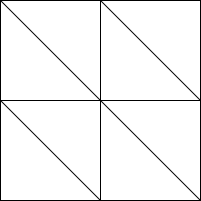
\includegraphics[width=\linewidth]
		{data/synthetic_meshes/square_tesselation_2tri_Dirac_delta_1_v9_f8_wireframe.png}
		\caption{R=1, wireframe}\label{fig:sq2.a}
	\end{subfigure}
	\begin{subfigure}[b]{0.32\linewidth}
		\includegraphics[width=\linewidth]
		{data/synthetic_meshes/square_tesselation_2tri_Dirac_delta_1_v9_f8_funcvals_0iter_crop.png}
		\caption{R=1, convolutions 0}\label{fig:sq2.b}
	\end{subfigure}
	\begin{subfigure}[b]{0.32\linewidth}
		\includegraphics[width=\linewidth]
		{data/synthetic_meshes/square_tesselation_2tri_Dirac_delta_1_v9_f8_funcvals_1iter_crop.png}
		\caption{R=1, convolutions 1}\label{fig:sq2.c}
	\end{subfigure}

	\bigskip
	\begin{subfigure}[b]{0.32\linewidth}
		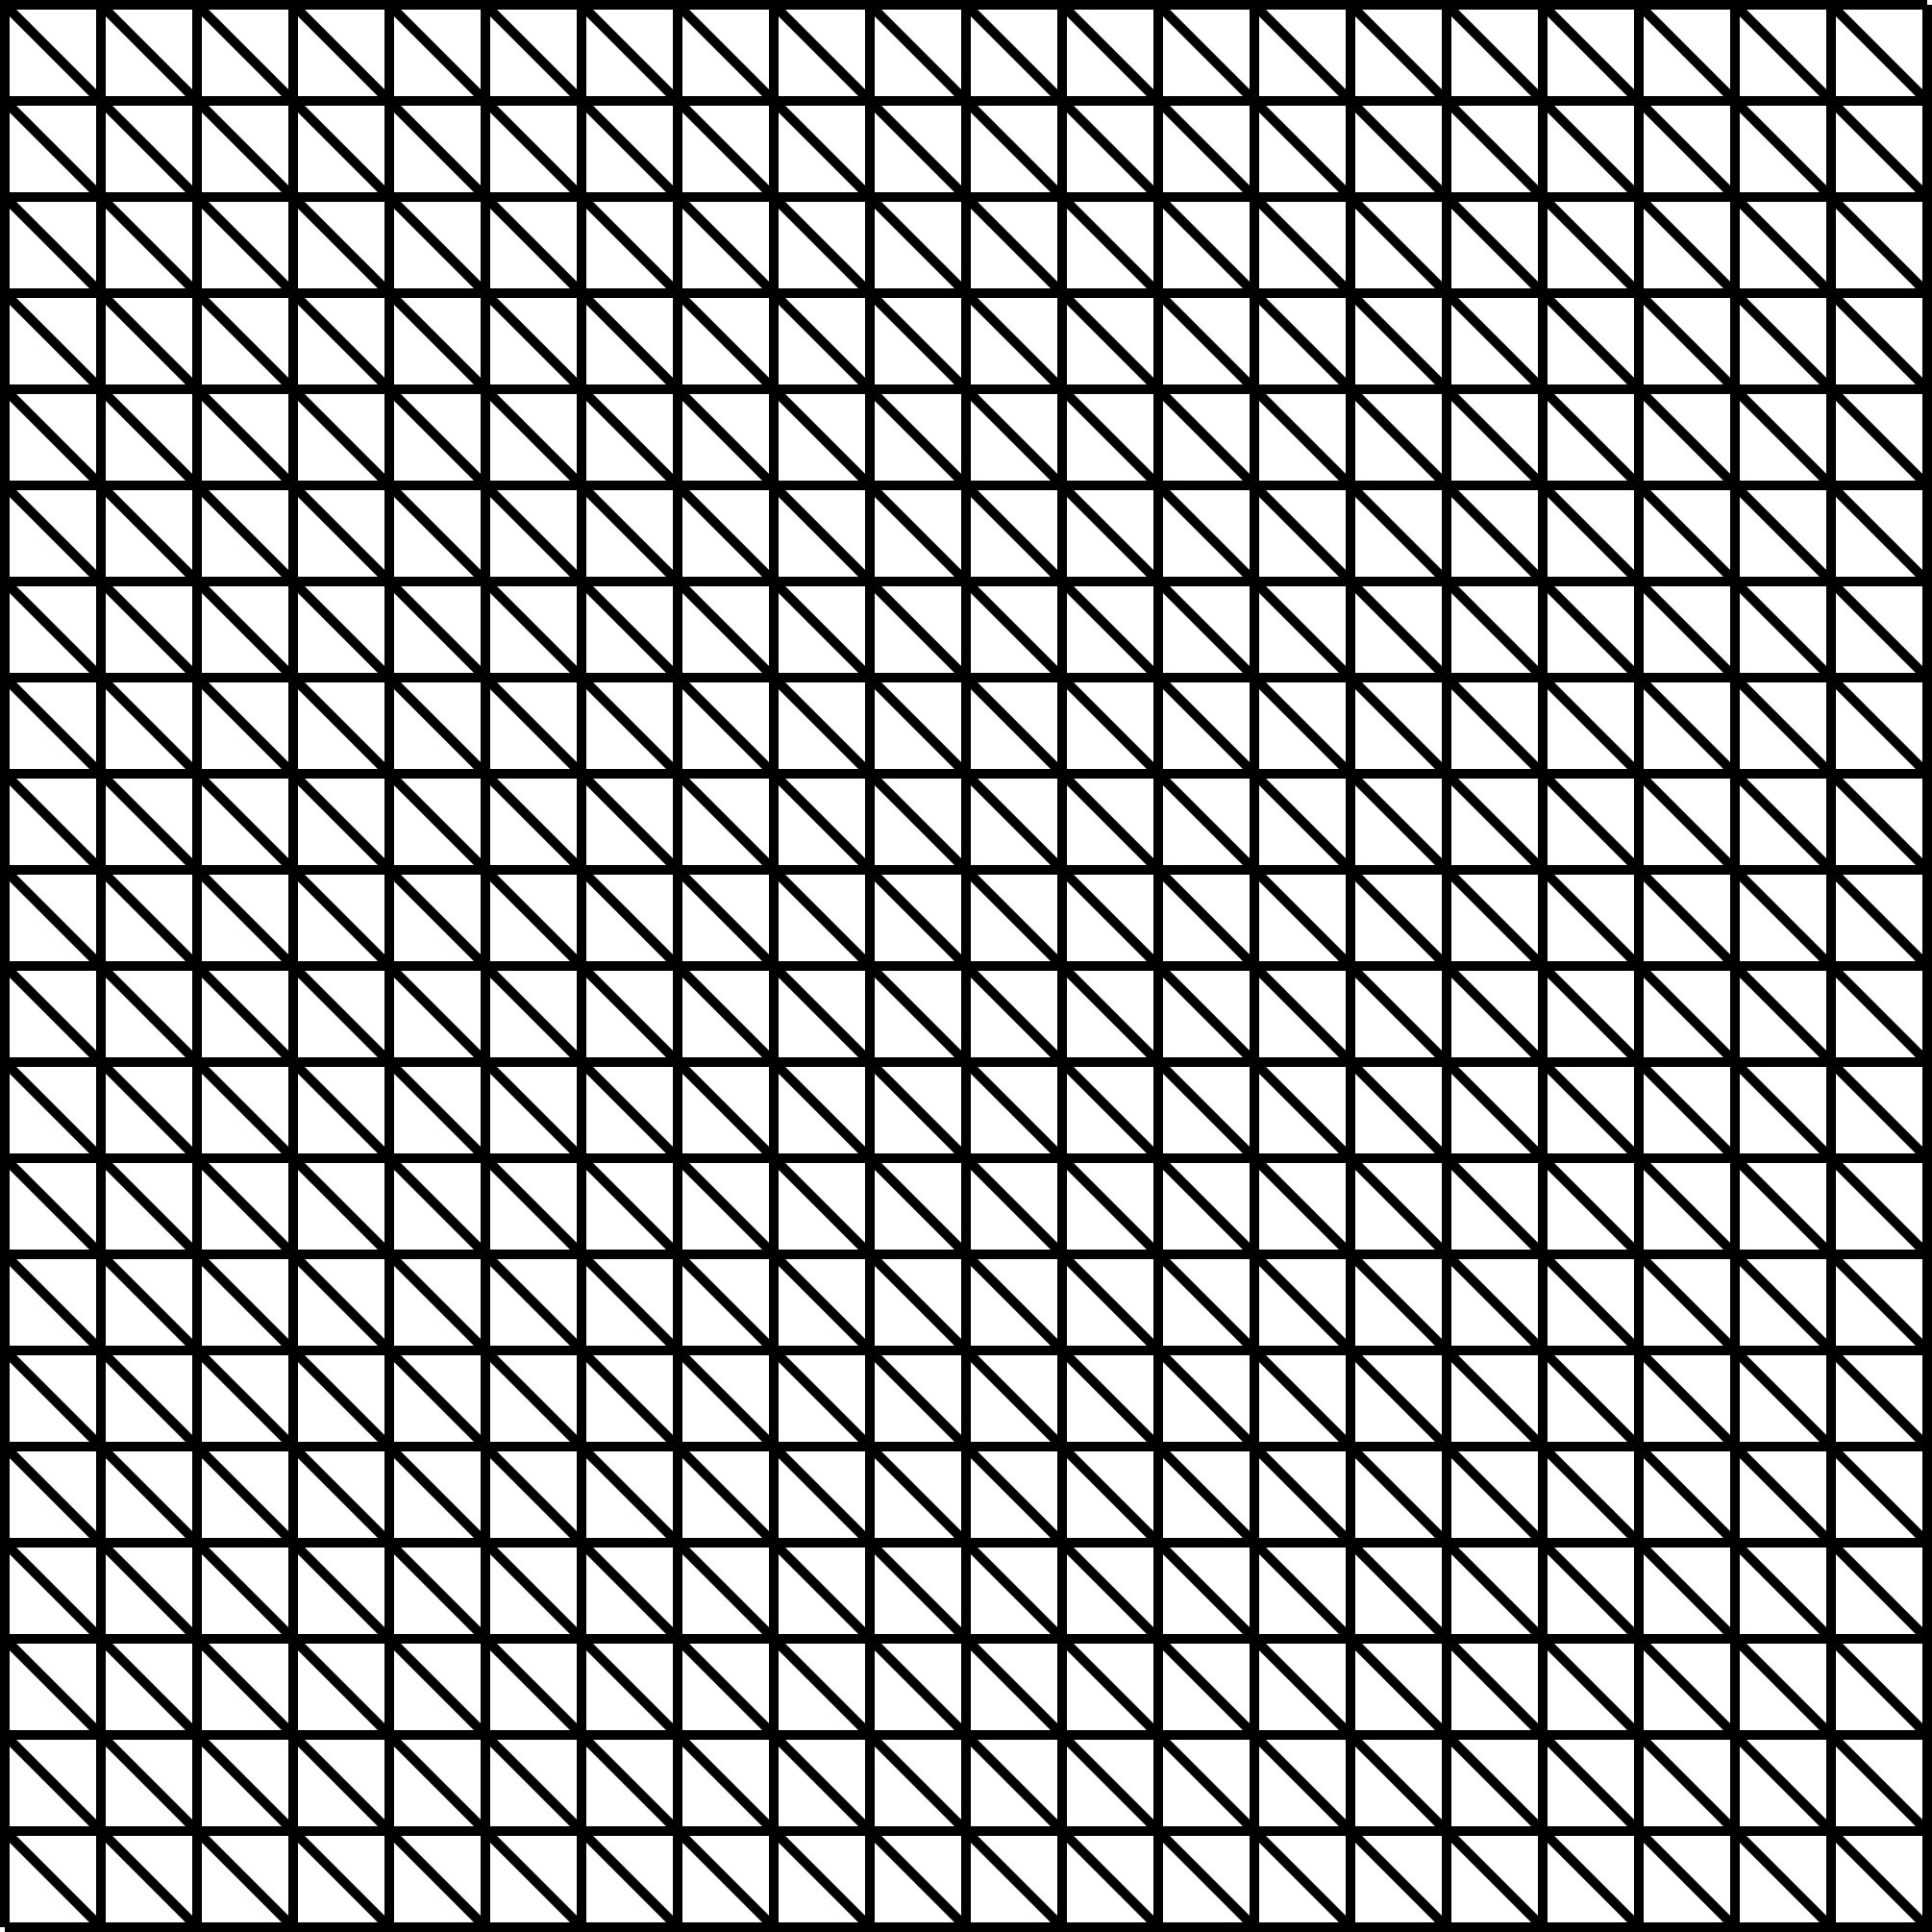
\includegraphics[width=\linewidth]
		{data/synthetic_meshes/square_tesselation_2tri_Dirac_delta_10_v441_f800_wireframe.png}
		\caption{R=10, wireframe}\label{fig:sq2.d}
	\end{subfigure}
	\begin{subfigure}[b]{0.32\linewidth}
		\includegraphics[width=\linewidth]
		{data/synthetic_meshes/square_tessellation_2tri_Dirac_delta_10_v441_f800_funcvals_0iter.png}
		\caption{R=10, convolutions 0}\label{fig:sq2.e}
	\end{subfigure}
	\begin{subfigure}[b]{0.32\linewidth}
		\includegraphics[width=\linewidth]
		{data/synthetic_meshes/square_tessellation_2tri_Dirac_delta_10_v441_f800_funcvals_100iter.png}
		\caption{R=10, convolutions 100}\label{fig:sq2.f}
	\end{subfigure}
	\caption[Six views, comparing two differently sized of bisected square tessellations]{Comparison of two differently sized bisected square tessellations, generated with parameters R set to 1 and 10: (a) R=1 in wireframe (b) R=1 colored by function value before convolving the filter (c) R=1 colored by function value after convolving the filter once (d) R=10 in wireframe (e) R=10 colored by function value before convoving the filter (f) R=10 colored by function value after convolving the filter 100 times.}
	\label{fig:sq2}
\end{figure}

%\todoResearch{Why does sq2 10 need 100 iters to match sq 1 at 1 iters?}

%
%
%
%
%\subsection{Square Tesselations, Four Triangles}

%
%
%
%
\subsection{Hexagonal Tesselation}
The synthetic mesh generator for hexagonal tessellations generates meshes which are characterized by rings of hexagons around one centeral hexagon, with each corner of a hexagon made adjacent to its center point, creating six equilateral triangles. The smallest mesh, generated with the parameter R equal to zero, is composed of only seven points and 6 faces, but grows quickly as summarized in table~\ref{tbl:hex}.

\begin{table}[ht]
\begin{tabular}{rrr}
\textbf{R} & \textbf{Points} & \textbf{Faces} \\
\hline
    0 &          7 &           6\\
    1 &         31 &          42\\
    3 &        133 &         222\\
   10 &      1,057 &       1,986\\
   30 &      8,557 &      16,746\\
  100 &     91,507 &     181,806\\
  300 &    814,507 &   1,625,406\\
1,000 &  9,015,007 &  18,018,006\\
3,000 & 81,045,007 & 162,054,006%
\caption{Summary of the Counts of Points and Faces for Increasing Parameters of the Hexagonal Tesselation Synthetic Mesh Generator\label{tbl:hex}}
\end{tabular}
\end{table}

Figure~\ref{fig:sq2} shows a comparison of
\begin{figure}[ht]
\ffigbox
	{\begin{subfigure}[b]{0.48\linewidth}
		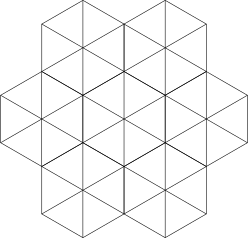
\includegraphics[width=1.0\linewidth,height=0.3\textheight,keepaspectratio]{data/synthetic_meshes/hexagonal_tessellation_Dirac_delta_1_v31_f42_wireframe.png}
		\caption{Hex v31\_f42 wireframe}\label{fig:hex.a}
	\end{subfigure}
	\begin{subfigure}[b]{0.48\linewidth}
		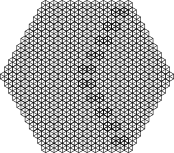
\includegraphics[width=1.0\linewidth,height=0.3\textheight,keepaspectratio]{data/synthetic_meshes/hexagonal_tessellation_Dirac_delta_10_v1057_f1986_wireframe.png}
		\caption{Hex v1057\_f1986 wireframe}\label{fig:hex.b}
	\end{subfigure}

	\bigskip
	\begin{subfigure}[b]{0.48\linewidth}
		\includegraphics[width=1.0\linewidth,height=0.3\textheight,keepaspectratio]{data/synthetic_meshes/hexagonal_tessellation_Dirac_delta_1_v31_f42_funcvals_0iter_crop.png}
		\caption{Hex v31\_f42 iter 0}\label{fig:hex.c}
	\end{subfigure}
	\begin{subfigure}[b]{0.48\linewidth}
		\includegraphics[width=1.0\linewidth,height=0.3\textheight,keepaspectratio]{data/synthetic_meshes/hexagonal_tessellation_Dirac_delta_10_v1057_f1986_funcvals_0iter_crop.png}
		\caption{Hex v1057\_f1986 iter 0}\label{fig:hex.d}
	\end{subfigure}

	\bigskip
	\begin{subfigure}[b]{0.48\linewidth}
		\includegraphics[width=1.0\linewidth,height=0.3\textheight,keepaspectratio]{data/synthetic_meshes/hexagonal_tessellation_Dirac_delta_1_v31_f42_funcvals_2iter_crop.png}
		\caption{Hex v31\_f42 iter 2}\label{fig:hex.e}
	\end{subfigure}
	\begin{subfigure}[b]{0.48\linewidth}
		\includegraphics[width=1.0\linewidth,height=0.3\textheight,keepaspectratio]{data/synthetic_meshes/hexagonal_tessellation_Dirac_delta_10_v1057_f1986_funcvals_200iter_crop.png}
		\caption{Hex v1057\_f1986 iter 200}\label{fig:hex.f}
	\end{subfigure}}
	{\caption[Synthetic Hexagonal Tessellations, Dirac delta function]{A synthetic hexagonal tessellation, subdivided by triangles, with a Dirac delta function applied: (a) v31 f42 wireframe (b) v1057 f1986 wireframe (c) v31 f42 colored by function value before filter (d) v1057 f1986 colored by function value before filter (e) v31 f42 colored by function value after 2 iterations (e) v1057 f1986 colored by function value after 200 iterations.
% All using the colorramp "Hot (improved)"~\cite[p.~???]{Brewer2003}~\cite[p.~19]{Giga17}, visualized using GigaMesh~\cite{Mara10}, exported as png after disabling the background grid [f7], maximizing the window, disabling screenshot cropping, as well as rejecting tiled rendering, finally cropping to content in GIMP.
	}\label{fig:hex}}
\end{figure}
\todoCitation{}


%
%
%
%
\subsection{Random Trigangulated Circles}
The synthetic mesh generator for random trigangulated circles generates meshes which are characterized by radially bounded, uniformally distributed, delaney triangulated, random meshes. Unlike the other generators, this requires two parameters, the radius R, and the number of points P. The smallest mesh,



generated with the parameter R equal to zero, is composed of only seven points and 6 faces, but grows quickly as summarized in table~\ref{tbl:hex}.

\begin{table}[ht]
\begin{tabular}{rrr}
\textbf{R} & \textbf{Points} & \textbf{Faces} \\
\hline
    0 &          7 &           6\\
3,000 & 81,045,007 & 162,054,006%
\caption{Summary of the Counts of Points and Faces for Increasing Parameters of the Hexagonal Tesselation Synthetic Mesh Generator\label{tbl:hex}}
\end{tabular}
\end{table}

Figure~\ref{fig:sq2} shows a comparison of
%\begin{figure}[ht]
\ffigbox
	{\begin{subfigure}[b]{0.48\linewidth}
		\includegraphics[width=1.0\linewidth,height=0.3\textheight,keepaspectratio]{data/synthetic_meshes/random_circle_tessellation_Dirac_delta_1_v11_f12_wireframe.png}
		\caption{R.Circ v11\_f12 wireframe}\label{fig:rcirc.a}
	\end{subfigure}
	\begin{subfigure}[b]{0.48\linewidth}
		\includegraphics[width=1.0\linewidth,height=0.3\textheight,keepaspectratio]{data/synthetic_meshes/random_circle_tessellation_Dirac_delta_10_v641_f1252_wireframe.png}
		\caption{R.Circ v641\_f1252 wireframe}\label{fig:rcirc.b}
	\end{subfigure}

	\bigskip
	\begin{subfigure}[b]{0.48\linewidth}
		\includegraphics[width=1.0\linewidth,height=0.3\textheight,keepaspectratio]{data/synthetic_meshes/random_circle_tessellation_Dirac_delta_1_v11_f12_funcvals_0iter.png}
		\caption{R.Circ v11\_f12 iter 0}\label{fig:rcirc.c}
	\end{subfigure}
	\begin{subfigure}[b]{0.48\linewidth}
		\includegraphics[width=1.0\linewidth,height=0.3\textheight,keepaspectratio]{data/synthetic_meshes/random_circle_tessellation_Dirac_delta_10_v641_f1252_funcvals_0iter.png}
		\caption{R.Circ v641\_f1252 iter 0}\label{fig:rcirc.d}
	\end{subfigure}

	\bigskip
	\begin{subfigure}[b]{0.48\linewidth}
		\includegraphics[width=1.0\linewidth,height=0.3\textheight,keepaspectratio,height=0.3\textheight,keepaspectratio]{data/synthetic_meshes/random_circle_tessellation_Dirac_delta_1_v11_f12_funcvals_0iter.png}
		\caption{R.Circ v11\_f12 iter 2}\label{fig:rcirc.e}
	\end{subfigure}
	\begin{subfigure}[b]{0.48\linewidth}
		\includegraphics[width=1.0\linewidth,height=0.3\textheight,keepaspectratio,height=0.3\textheight,keepaspectratio]{data/synthetic_meshes/random_circle_tessellation_Dirac_delta_10_v641_f1252_funcvals_10000iter.png}
		\caption{R.Circ v641\_f1252 iter 10,000}\label{fig:rcirc.f}
	\end{subfigure}}
	{\caption[Synthetic random vertices equally distributed per radius, Dirac delta function]{A synthetic circle filled with random vertices equaly distributed per radius, triangulated by Delauney method~\cite[p.~??]{todoCitation}, with a Dirac delta function applied: (a) v11\_f12 wireframe (b) v641\_f1252 wireframe (c) v11\_f12 colored by function value before filter (d) v641\_f1252 colored by function value before filter (e) v11\_f12 colored by function value after 2 iterations (f) v641\_f1252 colored by function value after 10,000 iterations.
%All using the colorramp "Hot (improved)"~\cite[p.~???]{Brewer2003}~\cite[p.~19]{Giga17}, visualized using GigaMesh~\cite{Mara10}, exported as png after disabling the background grid [f7], maximizing the window, disabling screenshot cropping, as well as rejecting tiled rendering, finally cropping to content in GIMP.
}\label{fig:rcirc}}
\end{figure}
\todoCitation{}
\todoResearch{Why and who equally distributed}



%
%
%
%
%
%
\section{Acquired Data}
\dots

%
%
%
%
\subsection{University Seal}
Unisiegel\_\- UAH\_\- Ebay-Siegel\_\- Uniarchiv\_\- HE2066-60\_\- 010614\_\- partial\_\- ASCII.ply
%\begin{figure}[ht]
	\begin{subfigure}[b]{0.32\linewidth}
		\includegraphics[width=\linewidth]{data/acquired_meshes/unisiegel_wireframe.png}
		\caption{wireframe}\label{fig:unisiegel.a}
	\end{subfigure}
	\begin{subfigure}[b]{0.32\linewidth}
		\includegraphics[width=\linewidth]{data/acquired_meshes/unisiegel_0iter.png}
		\caption{$c=0$}\label{fig:unisiegel.b}
	\end{subfigure}
	\begin{subfigure}[b]{0.32\linewidth}
		\includegraphics[width=\linewidth]{data/acquired_meshes/unisiegel_100iter.png}
		\caption{$c=100$}\label{fig:unisiegel.c}
	\end{subfigure}
	\caption[Three views of the Univeristy of Heidelberg Seal]{Three views of the Univeristy of Heidelberg seal (a) in wireframe, (b) colored by \gls{tMSIIf} value before convolving the filter, (c) colored by function value after convolving the filter 100 times.}
	\label{fig:unisiegel}
\end{figure}


%
%
%
%
\subsection{A Flat surface}
Flat surfaces have NOISE!
Figure~\ref{fig:ILATO}: ILATO\_1A\_SM2066-HE5-60\_070214\_merged\_GMO\_r1.00\_n4\_v256
%\begin{figure}[ht]
	\begin{subfigure}[b]{0.49\linewidth}
		\includegraphics[width=\linewidth]
		{data/acquired_meshes/ILATO_1A_SM2066-HE5-60_070214_merged_GMO_r1_n4_v256_wireframe.png}
		\caption{wireframe}\label{ILATO:bun.a}
	\end{subfigure}
	\begin{subfigure}[b]{0.49\linewidth}
		\includegraphics[width=\linewidth]
		{data/acquired_meshes/ILATO_1A_SM2066-HE5-60_070214_merged_GMO_r1_n4_v256_funcvals_0iter.png}
		\caption{$c=0$}\label{fig:buILATOn.b}
	\end{subfigure}
	
	\bigskip
	\begin{subfigure}[b]{0.49\linewidth}
		\includegraphics[width=\linewidth]
		{data/acquired_meshes/ILATO_1A_SM2066-HE5-60_070214_merged_GMO_r1_n4_v256_funcvals_1000iter.png}
		\caption{$c=1000$}\label{fig:ILATO.c}
	\end{subfigure}
	\begin{subfigure}[b]{0.49\linewidth}
		\includegraphics[width=\linewidth]
		{data/acquired_meshes/ILATO_1A_SM2066-HE5-60_070214_merged_GMO_r1_n4_v256_funcvals_3000iter.png}
		\caption{$c=3000$}\label{fig:ILATO.d}
	\end{subfigure}
	\caption[Four views of a flat surface]{Four views of a flat surface (a) in wireframe (b) colored by MSII function value before convolving the filter (c) colored by function value after convolving the filter 1,000 times (c) and after 3,000 times.}
	\label{fig:ILATO}
\end{figure}


%
%
%
%
\subsection{Stanford Bunny}
Figure~\ref{fig:bun}: http://graphics.stanford.edu/data/3Dscanrep/ (Stanford Bunny)
%\begin{figure}[ht]
	\begin{subfigure}[b]{0.32\linewidth}
		\includegraphics[width=\linewidth]
		{data/acquired_meshes/bun_zipper_edited_r1_n4_v256_wireframe.png}
		\caption{wireframe}\label{fig:bun.a}
	\end{subfigure}
	\begin{subfigure}[b]{0.32\linewidth}
		\includegraphics[width=\linewidth]
		{data/acquired_meshes/bun_zipper_edited_r1_n4_v256_funcvals_0iter.png}
		\caption{$c=0$}\label{fig:bun.b}
	\end{subfigure}
	\begin{subfigure}[b]{0.32\linewidth}
		\includegraphics[width=\linewidth]
		{data/acquired_meshes/bun_zipper_edited_r1_n4_v256_funcvals_100iter.png}
		\caption{$c=100$}\label{fig:bun.c}
	\end{subfigure}
	\caption[Three views of the Stanford Bunny]{Three views of the Stanford Bunny (a) in wireframe (b) colored by function value before convolving the filter (c) colored by function value after convolving the filter 100 times.}
	\label{fig:bun}
\end{figure}


%
%
%
%
%
%
\section{Evaluation}
\ldots

%
%
%
%
\subsection{Compute Times}

Figure~\ref{fig:computeTimesLP} shows how compute times increase linearly with both mesh size and number of iterations in a very predictable way when total compute time is at least 0.1 seconds, and less predictable for shorter periods do to the nature of thread optimization at the processor level and variable memory read times.\todoResearch{add formula for timing (or at least ref to it) here.}\todoResearch{process time noise at very fast speeds}
\begin{figure}[ht]
	\centering
	\includegraphics[width=1.0\linewidth,height=1.0\textheight,keepaspectratio]
		{figures/computeTimesLinespoints.png}
	\RawCaption{\caption[Compute Times - Linespoints]{Compute Times of Applying
		the	One-Ring Filter for Selected Numbers of Iterations onto Acquired and
		Synthetic 3D Meshes of Varying Sizes}
		\label{fig:computeTimesLP}}
\end{figure}

Figure~\ref{fig:computeTimesS} shows how compute times increase with both meshsize and number of iterations.\todoCitation{wikipedia Euler characteristic Polyhedra}
\begin{figure}[ht]
	\centering
	\includegraphics[width=1.0\linewidth,height=1.0\textheight,keepaspectratio]{figures/computeTimesScatter.png}
	\RawCaption{\caption[Compute Times - Scatter]{Compute Times for Different
		Hardware Configurations by increaseing Mesh Size and Filter Iterations}
		\label{fig:computeTimesS}}
\end{figure}

%
%
%
%
\subsection{Curious Trend, ratio goes to 2}

\begin{figure}[ht]
	\centering
	\includegraphics[width=1.0\linewidth,height=1.0\textheight,keepaspectratio]{figures/numFacesByVerticesGoTo2.png}
	\RawCaption{\caption[Ratio of Faces / Vertices]{Ratio of Faces to Vertices by
		Increasing Vertex Count}
		\label{fig:ratioFacesVertices}}
\end{figure}



%\subsection{Debossed H}
%In Figure \ref{fig:h}, we show a debossed capital letter H.\footnote{The H is
%as a nod to Heidelberg University and the cuniform script studied by the FCGL.}
%\begin{figure}[ht]
%\centering
%	\begin{subfigure}{.48\linewidth}
%		\centering
%		\resizebox{0.48\linewidth}{!}{\input{data/synthetic_meshes/h.tikz_labels.tex}}
%		\caption{HWireframe}\label{fig:h.a}
%	\end{subfigure}
%	\hfill
%	\begin{subfigure}{.48\linewidth}
%		\centering
%		\includegraphics[width=0.48\linewidth]{data/synthetic_meshes/h_colored.png}
%		\caption{HColored}\label{fig:h.b}
%	\end{subfigure}
%	\caption[A debossed H, which contains 22 vertices and 36 faces.]{A debossed H,
%	which contains 22 vertices and 36 faces: (a) wireframe (b) colored by the
%	relation to its distance to an underlying plane, in RdGy
%	colorramp~\cite[p.~???]{Brewer2003}~\cite[p.~19]{Giga17}, visualized using the
%	GigaMesh~\cite{Mara10} framework with triangle edges rendered.}\label{fig:h}
%\end{figure}
%To evaluate methods available for discrete surfaces, we can increase the number of vertices of our synthetic wedge using five iterations of the mid-edge subdivision scheme [PR97,HW99].~\cite[p.~38]{Mara12}

%\subsection{Mars Crater}
%Mars dataset crater as a Digital Terrain Models (DTMs) Mention in Mara 3.6
%Summary “Dali” inspired methodProcessing regular grids like Digital Terrain Models (DTMs) will gain dramatic performance increases using the estimator, while processing irregular grids with high curvatures will strongly benefit from precise computation of the volume integral invariant.~\cite[p.~143]{Mara12}

%
%
%
%
%
%
\section{Summary}
\dots

\chapter{Conclusions}
As of this writing, the fastest available GPGPU card available is the Quadro RTX 6000 which has 4,608 parallel processing cores and can perform at 16.3 TFLOPS~\cite{quadro6k}, up from the the previous 5000 model, which already had 3,702 and could perform at 11.2 TFLOPS~\cite{quadro5k}.

The fastest CPU commercially available as of this writing is the Intel Core i9-9980XE, which has 16 cores which each operate at 3.0GHz, and costs about \$2,300.
\todoCitation{cpu benchmarks}
%https://www.cpubenchmark.net/cpu.php?cpu=Intel+Core+i9-9980XE+%40+3.00GHz&id=3373


%
%
%
%
%
%
\section{Summary}

The goal of our experimentation was two-fold, analyzing the filter response on various kinds of \tdd{} as well as evaluating the performance of the parallel variant of \fors{t} algorithm. Therefore, we began in Section~\ref{ch6sSTDD} by analyzing the filter response when convolving the filter of over four different configurations of synthetic \tdd{}: the bisected square tessellation, the quadrisected square tessellation, the hexagonal tessellation, and the random triangulated disc, each with the \gls{ddf} applied as a scalar field.

Figure~\ref{fig:sq2} exposed the behavior of the anisotropic filter response traveling faster along the connections of more distant adjacent points. Figures~\ref{fig:sq4}~and~\ref{fig:hex} show the filter response exhibiting isotropic behavior as the density of the mesh increased, with more adjacent points per unit compared to the bisected square tesselation, while also reducing the overall variance in the length of edges. Figures~\ref{fig:rdisc} showed how the filter response appears to slow down when convolved over irregular meshes, more similar to acquired \tdd{}.

Next, in Section~\ref{ch6sATDD} we analyzed the filter response when convolving the filter of over three different examples of acquired \tdd{}: the partial model of the University of Heidelberg seal, the flat surface from ILATO, and the Stanford Bunny, each processed having been processed by \gls{tMSIIf}.

In Figure~\ref{fig:unisiegel} an error in computation was seen propagating across the image with each subsequent convolution. However, as that error stems from convolving the filter over ``unclean'' \tdd{}, the solution lies not with the filter, but with first processing the data with another tool, such as the ``Automatic Mesh Polishing'' provided by the GigaMesh framework.

In Figure~\ref{fig:ILATO}, the filter response efficacy diminishes,  seemingly having had its effectiveness compromised by convolving the filter over a scalar field with very low variance, highlighting another complexity of working with acquired \tdd{}, where one solution may be to set limits on the range of values visualized by the software.


%
%
%
%
%
%
\section{Future Work}
What they are and why I did not.
\begin{itemize}
	\item Implement in OpenCL to include all GPUs
	\item Implement in OpenMP to use multiple machines
	\item Implement in PThreads to exploit MIMP
	\item Pipelining memory reads/calculations exploit more concurrency
	\item Edge case handling: max mesh size in memory, Derive calculation for compute time per iteration by mesh size. Maybe find when load time is greater than iteration time
	\item support other file types
	\item Calculating edge length takes longest, so DO NOT DOUBLE EFFORT HERE
	\item Determine is using $\elm$ vs $\bar{\elm}$ has any effect, especially on one-ring neighborhood with a relatively large $\elm$ on mesh with a very small $\bar{\elm}$
	\item More analysis on \fors. it is my intuition that the un-isotropic nature of the filter is due to the speed at which information travels along longer edges.
	\item Apply the filter to multi-channel vector fields like RGB, however color-wheel based methods may be better From scetion
\label{ch2sTDDssFV}
	\item Implement Median and Mode version of filter (others based on what's foudn in 2d filter results)
	\item Implement more storage vs speed options
	\item explore using the inner angles $\alpha_i$ in stead of area for weighting
	\item instead of global min size, just choose a size, especially if not using sqrt to get edgelengths
	\item create more synthetic meshes with different scalar fields, Random, etc
	\item \ref{fig:speedup} Another trend is that for most configurations, speedup increases with increasing number of convolutions, seeming to converge to a certain number. More research must be done in order to determine why this may be, but it is possible that it is related to low-level memory optimization by the operating system.
	\item if neighborhood sizes vary widely, one large neighborhood can cause all other threads to wait. therefore, build in work sharing for big neighborhoods.
	\item improve efficency of parallel algorithm
	\item exploit errorInSource to speed up parallel algorithm
	\item at end of \label{ch5sCELPssASACEL} Conversely, in order to save nearly half\footnote{Scaling by half comes from the observation that as mesh density increases, the ratio of border to non-border edges dimensions, which discussed in more detail Appendix~\ref{apdx1}.} of that memory, one could store the value only once by implementing the control structures for detecting if an edge length has already been saved, then when retrieving the values, one could search for the edge length required at the cost of compute time. In the next section, we choose to implement the first, speedier method.
\end{itemize}


%
\appendix
\include{chapters/A1-Appendix}
%
\backmatter
\printindex
\printglossaries
\bibliography{thesis}{}
\bibliographystyle{plain}
\todoRemove{remove todoCitation from bibliography}
\todoStyle{should bibliographystyle be plain?}

\end{document}

